% HAMMER -- IEEE conference-format manuscript 
%
% Class: IEEEtran in conference mode, A4 paper, two columns (Overleaf's TeX Live ships IEEEtran).
% Bibliography: BibTeX, IEEEtran.bst, numbered citations.
%
% No venue has been chosen. No conference name, dates, copyright block, ISBN or
% IEEE-branded footer is inserted on purpose (see paper README).
\documentclass[conference,a4paper]{IEEEtran}

\IEEEoverridecommandlockouts

\usepackage{cite}
\usepackage{amsmath,amssymb,amsfonts}
\usepackage{graphicx}
\usepackage{textcomp}
\usepackage{xcolor}
\usepackage{booktabs}
\usepackage{array}
\usepackage{url}

\def\BibTeX{{\rm B\kern-.05em{\sc i\kern-.025em b}\kern-.08em
    T\kern-.1667em\lower.7ex\hbox{E}\kern-.125em X}}

% Shared notation (used from Stage 2 onward)
\newcommand{\hammer}{\textsc{HAMMER}}

\begin{document}

\title{Hybrid Academic Metadata Aggregator and\\
Evidence-Guided Author Entity Resolution System}

% Author names, department, institution and e-mail addresses are taken from the title-block
% image supplied by the project team. Supervisor / guide: not supplied, deliberately omitted.
\author{
\IEEEauthorblockN{Namit Lalwani}
\IEEEauthorblockA{\textit{Dept.\ of Information Technology}\\
\textit{KJ Somaiya School of Engineering}\\
\textit{Somaiya Vidyavihar University}\\
namit.l@somaiya.edu}
\and
\IEEEauthorblockN{Akshad Kedia}
\IEEEauthorblockA{\textit{Dept.\ of Information Technology}\\
\textit{KJ Somaiya School of Engineering}\\
\textit{Somaiya Vidyavihar University}\\
akshad.kedia@somaiya.edu}
\and
\IEEEauthorblockN{Nicholas Coutinho}
\IEEEauthorblockA{\textit{Dept.\ of Information Technology}\\
\textit{KJ Somaiya School of Engineering}\\
\textit{Somaiya Vidyavihar University}\\
nicholas.s@somaiya.edu}
\and
\IEEEauthorblockN{Sunil Shelke}
\IEEEauthorblockA{\textit{Dept.\ of Information Technology}\\
\textit{KJ Somaiya School of Engineering}\\
\textit{Somaiya Vidyavihar University}\\
sunil.shelke@somaiya.edu}
}

\maketitle

\begin{abstract}
Scholarly metadata is scattered across providers, and an aggregator must decide both whether two records describe the same work and whether a name denotes a particular person. We describe \hammer{}, an implemented aggregator that keeps the two decisions separate. For authors it retrieves candidate profiles from OpenAlex, extracts up to five evidence signals, combines them in a heuristic score that is not a probability, and applies conservative gates that end in automatic assignment, manual review or an unresolved result. We contribute no new algorithm. We contribute an evaluation design that separates provisional benchmark labels from independently verified labels, keeps every outcome in the denominators and plans the sample size from a label-free pilot, together with offline tooling validated by 591 tests, mutation checks and simulation. The independent verification this design requires has not been performed, so we report no verified accuracy. We report instead exploratory, benchmark-derived observations from 68 real queries of the LAGOS-AND benchmark (a 50-case smoke sample and 18 randomly selected cases). The profile carrying the benchmark ORCID was in the retrieved pool for 76\% and 72\% of the queries but was the provider's first candidate for only 44\% and 39\%. With name, institution and year supplied, 4 of 50 and 0 of 18 queries were assigned automatically: scores were high (median 0.88) but rarely separated from similarly named competitors. HAMMER's own top-one choice agreed with the benchmark label no more often than the provider's order (34\% and 33\% against 44\% and 39\%). These samples are small, clustered and benchmark-labelled, so they indicate where the approach is limited and do not estimate its accuracy.
\end{abstract}

\begin{IEEEkeywords}
author name disambiguation, entity resolution, scholarly metadata, candidate retrieval,
selective prediction, provenance
\end{IEEEkeywords}

\section{Introduction}
\label{sec:introduction}

Scholarly metadata is spread across many bibliographic providers. Open indexes such as OpenAlex expose works, authors and institutions at scale~\cite{priem2022openalex}, but the providers differ in what they cover, and coverage comparisons show that the differences depend on the task and on the sources compared~\cite{culbert2025openalexcoverage}. A record for the same publication may therefore be incomplete, formatted differently, or duplicated across sources, and its author list may be abbreviated, reordered or attached to different identifiers. An application that aggregates such records has to decide two separate questions.

The first is whether two records describe the same \emph{work}. This is a record-linkage and deduplication problem with a long statistical and practical history~\cite{fellegi1969recordlinkage,elmagarmid2007duplicate,forbes2024deduplicator}. The second is whether a name on a record, or a name typed by a user, refers to a particular \emph{person}. This is author name disambiguation, a mature field with several task formulations and a large literature~\cite{ferreira2012brief,rodrigues2024andreview,debonis2023graph}. The two questions use different evidence and carry different costs of error. A shared DOI is strong evidence that two records are the same work, whereas two researchers with the same or similar names may be different people, and one researcher may appear under several name forms. Treating a work-level match as if it settled a person-level question, or the reverse, hides the uncertainty that a user most needs to see.

This paper concerns the second question, in the setting of a scholarly metadata aggregator. We use the following terms consistently. \emph{Candidate retrieval} obtains a set of possible author profiles for a query. \emph{Ranking} orders that set. An \emph{identity decision} is the choice among three outcomes: automatic assignment of one candidate, manual review, or an unresolved result. These steps are not interchangeable. A retriever that never returns the correct profile cannot be rescued by any ranker or decision rule, and a ranker that places the correct profile first does not by itself justify assigning it automatically.

The literature treats the surrounding pieces separately. Benchmark studies evaluate clustering or assignment of publications to authors, typically with F1-style measures, and report that models trained on one dataset may generalize poorly to others~\cite{subramanian2021s2and,chen2023whoiswho}. General work on selective prediction supplies the vocabulary of coverage and risk for systems that may decline to answer~\cite{chow1970reject,elyaniv2010foundations,geifman2019selectivenet}. Deployed systems combine automatic disambiguation with human annotators~\cite{zhang2018aminerhitl}. Within the sources we reviewed, we did not identify a study that reports the retrieval stage and the selective assignment stage together, on the same frozen candidate pool, with manual-review, unresolved and provider-failure outcomes kept in the denominators. This is a statement about the limited search described in Section~\ref{sec:related}, not a claim that no such study exists.

We study this problem through \hammer{} (Hybrid Academic Metadata Aggregator and Evidence-Guided Author Entity Resolution System), an implemented application. \hammer{} aggregates metadata from several providers, normalizes and deduplicates publication records, and stores provenance for each source record. Its author-resolution component retrieves candidate author profiles from OpenAlex and scores them with five evidence signals: name similarity, institutional evidence, publication overlap, coauthor evidence and temporal compatibility. The signal weights are engineering defaults and are renormalized over the signals that are available; the resulting score ranks candidates and feeds a set of conservative decision gates, but it is a heuristic score and not a calibrated probability. When evidence is missing or a provider call fails, the system reports that state explicitly and does not treat it as evidence against a candidate.

\hammer{} does not propose a new disambiguation algorithm, and we make no claim of algorithmic novelty. Each ingredient it uses has prior art, and combining existing components does not by itself constitute a contribution to the method. The contribution we aim to establish is narrower: a provenance-aware workflow that keeps work-level matching separate from person-level decisions, together with an evaluation protocol that measures how its decision gates trade automatic precision against coverage. Our primary research question is:

\begin{quote}
\textbf{RQ2.} How effectively does \hammer{} retrieve author candidates, and how do its evidence-guided decision gates balance automatic assignment precision against coverage?
\end{quote}

We separate it into \textbf{RQ2a}, which asks how effectively the candidate retrieval process returns the expected author profile (Recall@$k$, mean reciprocal rank, candidate pool size, empty-result rate and candidate-pool mapping rate), and \textbf{RQ2b}, which asks how the decision gates affect the trade-off between the correctness of automatic assignments and automatic coverage (automatic precision, automatic coverage, manual-review and unresolved rates, selective risk and false automatic assignments). Precision and coverage are always reported together: a system that assigns few cases automatically cannot be called accurate without that coverage being visible, and a system that abstains on every case is not safe merely because it makes no wrong assignment.

The contributions of this paper, subject to the evidence presented in the later sections, are:
\begin{enumerate}
  \item An integrated architecture for scholarly metadata aggregation with source-level provenance, in which publication-level deduplication and author-level identity decisions are separate stages (Section~\ref{sec:architecture}).
  \item A staged author-resolution workflow, from candidate retrieval through evidence extraction and scoring to conservative decision gates, with explicit handling of missing and failed evidence and three outcomes: automatic assignment, manual review, and unresolved (Section~\ref{sec:methodology}).
  \item An evaluation protocol that reports retrieval effectiveness and selective resolution on one frozen candidate pool, controls for label and evidence leakage, and keeps uncertain and unresolved cases in the record (Section~\ref{sec:design}).
  \item Reproducible experimental artifacts: byte-level capture of provider responses with recorded hashes, and offline replay of the resolver from those captures (Section~\ref{sec:design}).
  \item Exploratory, benchmark-derived observations on 68 real queries that locate where the gates lose coverage (competition among similarly named candidates, not low scores) and that show the heuristic ordering of a pool doing no better than the provider's own order (Section~\ref{sec:results}).
\end{enumerate}

This manuscript reports a complete system and a fully specified evaluation, but not a verified accuracy. The independent identity-label audit on which the primary claims depend has not been performed, and no precision, recall or coverage figure is claimed as a property of the system. We report instead exploratory observations from 68 real queries (Section~\ref{sec:results}), labelled as benchmark-derived, small and clustered, and we state what they do and do not show.

The remainder of the paper is organized as follows. Section~\ref{sec:related} reviews related work and positions \hammer{} against it. Section~\ref{sec:architecture} describes the system architecture, Section~\ref{sec:methodology} the author-resolution method, and Section~\ref{sec:design} the experimental design and evaluation protocol. Sections~\ref{sec:results}--\ref{sec:conclusion} cover results, discussion, threats to validity, and conclusions.

\section{Related Work}
\label{sec:related}

This section reviews seven strands of work that bear on \hammer{}: record linkage, author name disambiguation, benchmarks and ground truth, candidate generation and assignment, evidence combination, selective prediction with human review, and metadata integration with provenance. It is built from a literature inventory compiled for this project. Most entries were checked at the level of bibliographic record and abstract, and a minority were read more closely; statements below that something was not found refer only to that inventory and are not evidence that nothing exists.
The inventory is not a systematic review. It was compiled on 19 November 2026 from the project's earlier audit documents and a small targeted extension of exploratory web searches and bibliographic-record look-ups (Crossref, arXiv, Zenodo, JMLR and PMLR pages); no pre-registered protocol, database export or dual screening was used, and no count of screened records was kept. Scopus, Web of Science, Google Scholar, dblp and Semantic Scholar were not searched. The characterisations of S2AND, WhoIsWho, CONNA, HUMO, r-HUMO and LAGOS-AND below were checked against their abstracts and the readable parts of their text on 20 November 2026; the JASIST version of the LAGOS-AND paper could not be read, so its description rests on the arXiv preprint and the Zenodo record.

\subsection{Record Linkage and Work-Level Matching}
Fellegi and Sunter cast record linkage as a decision among links, non-links and possible links under a probabilistic model of field agreement~\cite{fellegi1969recordlinkage}, and later surveys of duplicate-record detection build on that framing~\cite{elmagarmid2007duplicate}. Work-level deduplication remains an active applied task, for example in the preparation of systematic reviews~\cite{forbes2024deduplicator}. These methods ask whether two \emph{records} describe the same item. They do not decide whether a name refers to a given \emph{person}, which is why \hammer{} keeps the two stages apart. \hammer{}'s fixed-weight score has no estimated match and non-match probabilities and is not calibrated, so it should not be read as a Fellegi--Sunter model, even though its three outcomes resemble the three decision regions. Publication deduplication is part of the system but is not the subject of the research questions studied here.

\subsection{Author Name Disambiguation}
Author name disambiguation (AND) has been surveyed repeatedly~\cite{ferreira2012brief,debonis2023graph}. A recent review of 211 documents groups methods into grouping (similarity and clustering) and assignment (classification) families~\cite{rodrigues2024andreview}. Early learning-based work treated citation-level disambiguation as supervised classification~\cite{han2004twosupervised}, domain-specific methods were developed for MEDLINE~\cite{torvik2009authority}, and probabilistic frameworks were proposed for digital libraries~\cite{tang2012unified}.

More recent systems combine several sources and signals. PubMed Computed Authors provides an open resource of disambiguated PubMed author names~\cite{tian2024pubmedcomputedauthors}. AggAND aggregates several large scholarly databases to improve PubMed author name disambiguation~\cite{zhang2021aggand}. Boukhers and Asundi disambiguate DBLP authors with neural representations of names, coauthors and publication text~\cite{boukhers2024deepdblp}, and Choi et al.\ select a disambiguation scheme according to the metadata available from heterogeneous academic sites~\cite{choi2024heterogeneoussites}. Aggregating sources, using several evidence types, and adapting to available metadata therefore all have prior art, and \hammer{} claims none of them as new.

\subsection{Benchmarks and Ground Truth}
Benchmarks differ in task form and in how identity labels are obtained. S2AND consolidates eight existing datasets into a common format and reports that models trained on a single dataset may generalize poorly to others~\cite{subramanian2021s2and}. WhoIsWho provides a benchmark of more than one million papers with an evaluation task for real-time assignment of new papers to candidate authors~\cite{chen2023whoiswho}. GSD1900 offers 1,900 MEDLINE publication pairs for pairwise evaluation~\cite{vishnyakova2019gsd1900}. LAGOS-AND derives its gold-standard data, including a block subset, from ORCID and DOI evidence~\cite{zhang2023lagosand}, and the version used in this work was released for MAG and OpenAlex author identifiers~\cite{zhang2022lagosandv2}. The quality of AND datasets and the way AND is evaluated have themselves been examined~\cite{muller2017datasets,kim2018dblp}.

These resources are not interchangeable with the task studied here. Most formulate AND as clustering, pairwise classification or paper-to-person assignment, whereas \hammer{} resolves a query, a name with optional context, to an author profile in an external provider's index. Labels derived from ORCID linkage deserve particular care in our setting: the identifier that defines the label may also be present in the candidate source being evaluated, so agreement on it is a provisional matching mechanism and not independent identity truth. We return to this circularity in Sections~\ref{sec:design} and~\ref{sec:threats}.

\subsection{Candidate Generation and Assignment}
Entity-resolution pipelines commonly restrict the pairs to be compared through blocking and filtering, a stage that has its own survey literature~\cite{papadakis2020blocking}. In author disambiguation, assignment of a new paper to existing candidate authors is an explicit task in WhoIsWho~\cite{chen2023whoiswho}. CONNA goes a step further: it matches a paper to its best candidate person and then decides whether to assign the paper or to create a new person, with the matching and decision components fine-tuned jointly by reinforcement learning after separate training~\cite{chen2020conna}. The decision after ranking is therefore not new, and \hammer{}'s gates are best seen as a conventional, rule-based variant.

\hammer{} draws its candidates from OpenAlex~\cite{priem2022openalex}. We treat an OpenAlex author identifier as a provider profile and not as a verified person. Because the pool is whatever the provider returns for a query, it bounds what any later stage can achieve: if the expected profile is absent, ranking and decision rules cannot recover it. Retrieval effectiveness is therefore a separate question (RQ2a). Within the inventory we did not find an AND study that reports a retrieval-stage measure such as Recall@$k$ separately from final assignment quality; the summaries available to us for CONNA and WhoIsWho describe assignment accuracy and do not mention one.

\subsection{Evidence Signals and Their Combination}
Prior systems rely on name, coauthor, publication-text, venue and affiliation evidence in various combinations~\cite{boukhers2024deepdblp,zhang2021aggand,tian2024pubmedcomputedauthors}, and the choice of how to weigh them may be learned or rule-based. In the probabilistic tradition the weights come from estimated agreement and disagreement probabilities~\cite{fellegi1969recordlinkage,tang2012unified}. \hammer{} instead uses fixed engineering weights that are renormalized over the available signals. These weights have not been calibrated or validated, and because candidates may be scored over different signal sets, their scores are not always directly comparable. We state this as a limitation of the method and not as a design virtue (Section~\ref{sec:methodology}).

Institutional evidence deserves a separate note. Resolving raw affiliation strings to organization identifiers is a distinct, tool-supported task~\cite{duran-silva-etal-2024-affilgood,kallipoliti2025affro}. Such tools could supply institutional evidence to an author resolver, but the present work does not evaluate them.

\subsection{Selective Prediction and Human Review}
A predictor that may decline to answer trades coverage for lower error on the answers it gives. This reject-option framing goes back to Chow~\cite{chow1970reject}, was developed theoretically for selective classification~\cite{elyaniv2010foundations}, extended to deep networks with an integrated reject option~\cite{geifman2019selectivenet}, and has been surveyed more recently~\cite{hendrickx2024reject}. Risk and coverage are its standard evaluation quantities, and we adopt that vocabulary for RQ2b. The literature is general, and we did not find it applied to author identity with an explicit manual-review and unresolved split.

Human review in disambiguation is also established. AMiner combines clustering, maintenance and human annotators in the loop~\cite{zhang2018aminerhitl}. For entity resolution more generally, HUMO and r-HUMO divide the workload between machine and human to meet precision and recall targets~\cite{chen2018humo,hou2020rhumo}, and CrowdER uses crowdsourcing to resolve uncertain pairs~\cite{wang2012crowder}. \hammer{}'s manual-review outcome is a routing decision to a human, and the system gives no guarantee on the quality of what it assigns automatically; whether the gates achieve useful precision at useful coverage is an empirical question for RQ2b.

\subsection{Metadata Integration and Provenance}
OpenAlex is an open index of scholarly works, authors, venues, institutions and concepts~\cite{priem2022openalex}. Source coverage differs and depends on the task, and comparisons restricted to works shared by several indexes do not establish global coverage~\cite{culbert2025openalexcoverage}. Combining several databases has been used to improve author disambiguation~\cite{zhang2021aggand,choi2024heterogeneoussites}. The database literature gives provenance a formal treatment in terms of why- and where-provenance~\cite{buneman2001whyandwhere}. \hammer{} records, for each stored publication and candidate, which source supplied it and which evidence supported a decision. We use ``provenance'' in this practical sense and do not claim that the system implements the formal notions.

\subsection{Summary and Positioning}
Table~\ref{tab:literature} summarizes the works discussed. In short, AND is a mature field with several task forms, and multi-source evidence, an assign-or-new decision, human review and risk--coverage evaluation each exist separately. The gap we pursue is narrower than any technique. Within the sources reviewed, it is not established that prior work reports retrieval-stage recall and selective automatic-assignment precision against coverage together, on one frozen candidate pool, with manual-review, unresolved, empty-pool and provider-failure outcomes counted in the denominators. This is a statement about reporting and evaluation design. It is not a claim that \hammer{} is more accurate than any listed system, and no such comparison is made.

% Rows summarise the cited records. S2AND, WhoIsWho, CONNA, HUMO and r-HUMO were checked against abstract and readable text on 20 Nov 2026 (REFERENCE_VERIFICATION.md);
% the other rows rest on abstract-level or bibliographic-record readings. Cells saying "not compared" mean the cited work reports no measure that can be set beside HAMMER's.
\begin{table*}[t]
\caption{Representative prior work and its relation to \hammer{}. Task form, evidence and evaluation are as described by the cited sources.}
\label{tab:literature}
\centering
\footnotesize
\renewcommand{\arraystretch}{1.15}
\begin{tabular}{@{}p{0.15\textwidth}p{0.21\textwidth}p{0.19\textwidth}p{0.16\textwidth}p{0.19\textwidth}@{}}
\toprule
\textbf{Work} & \textbf{Task form} & \textbf{Evidence or ground truth} & \textbf{Evaluation family} & \textbf{Relation to \hammer{}} \\
\midrule
Fellegi and Sunter~\cite{fellegi1969recordlinkage} & Record-pair linkage with link, non-link and possible-link decisions & Probabilistic model over field agreement & Decision error rates & Foundation for the work-level layer; \hammer{}'s score is not a fitted probabilistic model \\
Rodrigues et al.~\cite{rodrigues2024andreview} & Review; grouping versus assignment families & Literature (2003--2022) & Not applicable & Taxonomy used to place \hammer{} \\
S2AND~\cite{subramanian2021s2and} & Clustering of author mentions across eight harmonised datasets & Existing dataset labels & Cluster-level F1 & Not compared: no candidate retrieval or abstention \\
WhoIsWho~\cite{chen2023whoiswho} & Benchmark with a real-time assignment task, more than one million papers & Curated benchmark labels & F1, AUC and MAP, by task & Closest task form; \hammer{} resolves a query to a provider profile, not a paper to a person \\
CONNA~\cite{chen2020conna} & Match a paper to the best existing person, then assign or create a new person & Two datasets; deployed on AMiner & F1 & Precedent for a decision stage after ranking \\
AMiner~\cite{zhang2018aminerhitl} & Clustering, maintenance and human annotators in the loop & Deployed system data & Not compared & Precedent for human review in the loop \\
AggAND~\cite{zhang2021aggand}; PubMed Computed Authors~\cite{tian2024pubmedcomputedauthors} & Disambiguation of PubMed author names with additional databases or multiple signals & PubMed-based datasets & Pairwise accuracy, F1 & Multi-source evidence has prior art; biomedical scope \\
Choi et al.~\cite{choi2024heterogeneoussites} & Scheme chosen according to metadata available from several academic sites & Non-public data & Not compared & Metadata-conditioned evidence has prior art \\
LAGOS-AND~\cite{zhang2023lagosand,zhang2022lagosandv2} & Gold-standard blocks of author records & ORCID and DOI linkage & Dataset, not a method & Benchmark candidate; labels are provisional (Section~\ref{sec:design}) \\
HUMO~\cite{chen2018humo}; r-HUMO~\cite{hou2020rhumo} & Machine--human workload split for entity resolution with quality targets & Entity-resolution datasets & Precision and recall targets against human cost & Quality-controlled review exists; \hammer{} offers no such guarantee \\
Selective classification~\cite{chow1970reject,elyaniv2010foundations,geifman2019selectivenet} & Predictors that may abstain & General classification & Risk--coverage & Supplies the evaluation vocabulary used for RQ2b \\
\bottomrule
\end{tabular}
\end{table*}


\section{HAMMER System Architecture}
\label{sec:architecture}

\hammer{} is an implemented application: a Python service built on FastAPI with an SQLite relational store, a persistent vector index, and a React front end. This section describes the components that exist in the code base and says which of them take part in the author-resolution experiment of Section~\ref{sec:design}. Many do not, and the description of a component is not a claim that it was evaluated. Fig.~\ref{fig:architecture} gives the overview and Table~\ref{tab:components} lists responsibilities.

The architecture has two levels that share no scores. The \emph{work level} decides whether provider records describe the same publication. The \emph{person level} proposes provider author profiles for a name and decides whether one of them may be assigned. Publication-matching outputs, such as a merged record's confidence field, are not inputs to the author decision, and author scores are not inputs to deduplication.

\begin{figure*}[t]
\centering
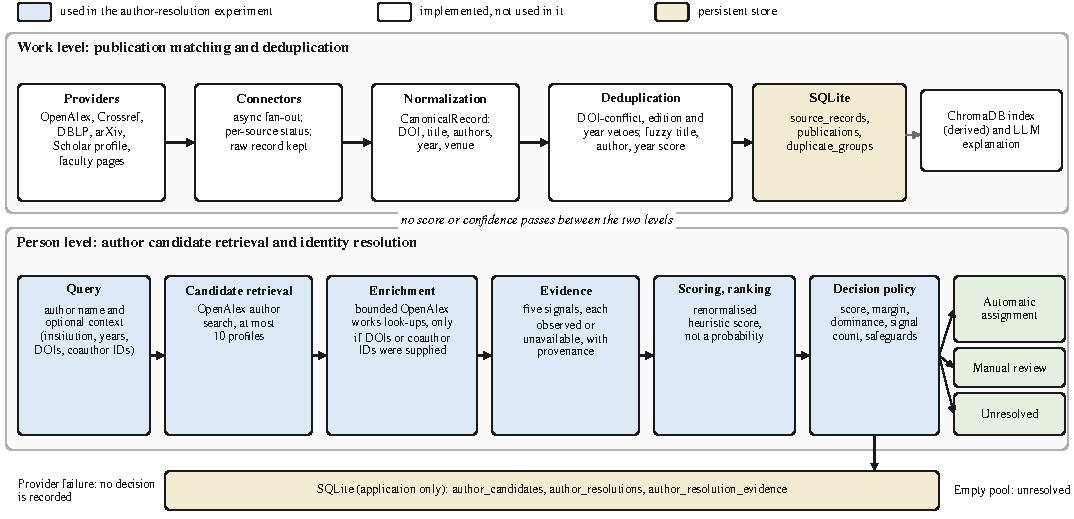
\includegraphics[width=\textwidth]{figures/architecture.pdf}
\caption{\hammer{} architecture. The work level (top) and the person level (bottom) are separate pipelines. Blue boxes take part in the author-resolution experiment; white boxes are implemented but are not used in it. The offline replay reads captured provider responses and neither reads nor writes the databases. Regenerate with \texttt{figures/make\_figures.py}.}
\label{fig:architecture}
\end{figure*}

\begin{table*}[t]
\caption{Components, responsibilities and role in the author-resolution experiment.}
\label{tab:components}
\centering
\footnotesize
\renewcommand{\arraystretch}{1.12}
\begin{tabular}{@{}p{0.17\textwidth}p{0.53\textwidth}p{0.22\textwidth}@{}}
\toprule
\textbf{Component} & \textbf{Responsibility} & \textbf{In the experiment?} \\
\midrule
Connectors & Fetch publication records from OpenAlex, Crossref, DBLP and arXiv, from cached Google Scholar profile pages for manually mapped authors, and from a configured faculty-page scraper; return records plus a per-source status & No \\
Normalization & Map each raw record to a canonical record (DOI, title, authors, year, venue, citations, raw JSON) & No \\
Deduplication & Decide whether two records are the same work; merge by source priority & No \\
Relational store & Keep raw source records, merged publications with per-field source attribution, duplicate groups, similarity logs, and author candidates, resolutions and per-signal evidence & No (replay uses no database) \\
Candidate retrieval & Query the OpenAlex authors endpoint and parse profiles into candidates & Yes \\
Enrichment & Bounded OpenAlex works look-ups that supply publication and coauthor evidence; coauthor evidence is supported in general but cannot be obtained on LAGOS-AND & Yes (publication evidence in C1x only; no coauthor evidence) \\
Evidence, scoring & Extract five signals per candidate and combine them into a heuristic score; on LAGOS-AND at most four can be observed, because coauthor identifiers are absent & Yes (at most four signals) \\
Decision policy & Apply score, margin, dominance, signal-count and safeguard rules; return one of three outcomes & Yes \\
Manual review & API and interface for a reviewer to select a candidate or mark the query unresolved & No (implemented; not exercised by the offline replay) \\
Vector index, LLM explanation & Rebuildable ChromaDB projection of canonical publications; optional Gemini explanation with citation containment & No; not shown to affect decisions \\
Capture and replay & Record each OpenAlex response with a hash; replay the resolver offline from the records & Yes \\
\bottomrule
\end{tabular}
\end{table*}

\subsection{Scholarly Metadata Acquisition}
Each connector implements one interface that returns a list of records and a status dictionary, and records a failure in the status instead of raising it. Per-source switches select the active connectors, and a configurable timeout bounds each call (ten seconds by default). A fixed source-priority order (Crossref, OpenAlex, DBLP, arXiv, Scholar, faculty page) decides which source supplies a field when records are merged. The raw response is stored with each source record.

Acquisition is not identity verification. A publication record carries author name strings, and the connector layer does not decide whether any name refers to a particular person. The author-resolution experiment uses only the OpenAlex authors and works endpoints (Section~\ref{sec:candidates}). The other connectors, the Scholar cache and the faculty scraper take no part in it.

\subsection{Normalization and Canonical Publication Records}
Normalization converts each provider record into one canonical form before comparison. HTML tags are stripped from titles and abstracts, DOIs are lower-cased with resolver prefixes removed, a four-digit year is extracted, author lists are parsed into name strings, and the citation count is coerced to an integer. A deterministic canonical identifier is derived from the DOI when one exists and otherwise from a hash of the source identifier and the normalized title.

The relational store keeps three views of a publication: the raw source record exactly as received, the merged canonical publication with the source that supplied each field (DOI, abstract, venue, citations) and the list of contributing sources, and a duplicate-group table that maps a merged publication to its source records. Source identifiers and raw JSON therefore survive merging.

\subsection{Publication Matching and Deduplication}
Deduplication answers a work-level question: do two records describe the same publication? It compares records pairwise after a cheap blocking step. Deterministic checks can veto or force a merge: conflicting valid DOIs forbid a merge, an identical DOI forces one, explicit conflicting edition markers (for example first and second edition) forbid one, and a year gap of four or more without a matching DOI forbids one. Remaining pairs receive a weighted similarity of title, author keys and year, which is compared with a threshold that depends on the pair of sources, and a title-similarity floor stops distinct works that share keywords from merging. Pairs whose score exceeds a logging threshold are written to an audit table with the merge decision. Groups are formed by union-find.

The output is a merged publication with a confidence field that is set by the number of contributing records, not by an estimate of correctness. It describes document equivalence only. It is not an identity confidence and is not used by the author resolver. Deduplication is not the subject of the research questions studied here, and no deduplication result is reported.

\subsection{Author Candidate Retrieval}
\label{sec:candidates}
Candidate retrieval produces hypotheses and nothing more. The candidate service queries the OpenAlex authors endpoint for a name and parses each returned object into a candidate profile: the provider's author identifier, display name and aliases, affiliations (institution name, OpenAlex institution identifier and ROR identifier where present), works count, citation count, the first and last year in the profile's yearly counts, and the raw payload. Malformed items, and items without an identifier or a non-blank display name, are dropped, and duplicate identifiers are removed in first-seen order. A returned identifier identifies a provider profile. It does not establish that the profile is the person the user meant, and it does not establish identity in any other source.

Retrieval has three distinguishable outcomes: a pool of candidates, a successful empty response, and a failure (timeout, request error, rate limit, HTTP error, malformed body, empty query, or an input that looks like an institution and is refused). A failure is never reported as an empty pool. The pool holds at most ten profiles from a single page.

Retrieval, ranking and assignment are separate steps. The order in which the provider returns candidates is the order used for the retrieval metrics. Ranking happens only after evidence extraction and uses the heuristic score of Section~\ref{sec:signals}. Assignment is a further step governed by the decision policy. Separately, the publication-search path contains an older candidate picker with its own score and automatic-selection rule; it is not the resolver described here and is not evaluated.

\subsection{Evidence Enrichment and Decision Workflow}
Evidence extraction, scoring and the decision policy are pure functions: they read a candidate and the query context and never touch the network, the database or the vector index. The only component that contacts OpenAlex for works-derived evidence is the enrichment service, and it does so only when the query supplies the input that makes a retrieval useful. If the query lists publication identifiers (DOIs or OpenAlex work identifiers, at most fifty), one look-up resolves their authorships. If it lists coauthor OpenAlex author identifiers, a bounded sample of each candidate's works (at most two pages of one hundred, with an explicit sort order) supplies that candidate's coauthors. An enrichment failure never fails the pool: it is recorded against the affected signal as unavailable.

The workflow therefore runs: candidate retrieval, optional enrichment, evidence extraction, scoring and ranking, and the decision policy of Section~\ref{sec:policy}, which yields \emph{automatic assignment}, \emph{manual review}, or \emph{unresolved}. In the application, a reviewer may then select one candidate or mark the query unresolved. That reviewer decision is stored as a separate status next to the algorithmic assessment, and each response states whether the decision came from the algorithm or a reviewer. An automatic assignment creates an internal author record linked to the OpenAlex profile with a note that the link is not cross-source proof, and the record is labelled an engineering heuristic and not a confidence.

\subsection{Provenance and Traceability}
We describe only what the code stores. Each source record keeps its raw provider response. A merged publication records which source supplied each of its fields and which sources contributed. Each author candidate keeps the raw provider payload and any retrieved enrichment, with retrieval time. For each candidate and signal, the evidence table stores the availability, the signal status, the normalized score, the raw comparison values, an explanation string, the provenance of the query-side and candidate-side inputs, the effective renormalized weight and the weighted contribution. Each resolution stores the top and second score, the margin, the dominance ratio, the decision reason, and the versions of the resolver, scoring and threshold configurations.

\emph{Implementation limitation.} The schema defines a per-source authorship table intended for authorship provenance, but we found no application code that populates it. Authorship-level provenance is therefore not available from the stored data, and we make no claim that it is. For the experiment, traceability is provided at file level by the capture toolkit (Section~\ref{sec:design}): each provider response is saved with a SHA-256 hash before the next request, and the replay verifies every hash before use.

\subsection{Scope of the Experiment}
Only the person-level components marked as used in Fig.~\ref{fig:architecture} take part in the experiment, and not all five evidence signals do: coauthor evidence cannot be observed on this benchmark (Section~\ref{sec:signals}). The manual-review API and interface are implemented but are not part of the automated offline replay; the experiment scores the algorithmic outcome only and does not evaluate reviewer behaviour. The replay reads captured OpenAlex responses and does not use the relational store, the vector index or the language model. The application's candidate endpoint also returns topical retrieval hits and a model-generated explanation next to the candidates, and the code states that they do not alter the deterministic decision. We have not tested whether they help or hurt identity resolution, and no such claim is made.

\section{Methodology}
\label{sec:methodology}

This section specifies the author-resolution method at the level needed to reproduce it. Every constant below was read from the committed configuration and code. The weights and thresholds are engineering defaults chosen by the developers. They were not learned from data, and they have not been calibrated or validated against independent labels.

\subsection{Task Definition}
\label{sec:task}
A \emph{query} $q=(n,\kappa)$ is a printed author name $n$ with an optional context $\kappa$ (Section~\ref{sec:leakage}). The \emph{provider catalog} is the set of author profiles in OpenAlex. A \emph{candidate} is a provider profile returned for $q$, and the \emph{candidate pool} $C(q)=(c_1,\dots,c_m)$, $m\le 10$, is the ordered list the provider returns. The \emph{expected identity} $g(q)$ is the person the query is meant to denote. It is defined by the benchmark's identity group and is provisional until audited (Section~\ref{sec:design}). A profile is \emph{mapped} to $g(q)$ if it represents that person, and a person may be mapped to several profiles because providers fragment identities.

Five operations are kept separate. \emph{Candidate retrieval} produces $C(q)$. \emph{Candidate ranking} orders $C(q)$ by a heuristic score. \emph{Identity assignment} selects one candidate as the answer. \emph{Abstention} withholds assignment and routes the query to \emph{manual review} when some candidate is plausible, or leaves it \emph{unresolved} when none is. A provider failure produces no decision at all. The unit of analysis is the query, with one primary query per identity group. Queries from the same name block are not independent observations (Section~\ref{sec:design}).

\subsection{Candidate Retrieval Configurations}
\label{sec:retrieval}
Two retrieval configurations are defined. Both request one page of at most ten profiles from the OpenAlex authors endpoint.

\textbf{R0} sends the trimmed raw query as \texttt{filter=display\_name.search:}$n$. It applies no normalization and no fallback. R0 exists only in the capture toolkit; the application never issues it.

\textbf{R2} is the application's committed strategy. It first applies the query cleaner, which normalizes Unicode (NFC), collapses whitespace, and joins ``Le'' or ``La'' to a following capitalized alphabetic token of more than two letters (for example ``Le Cun'' becomes ``LeCun''), and then sends the same filter. If, and only if, that primary request succeeds with no valid candidate and the cleaned query contains an initial (a single letter followed by a period), a second request uses \texttt{search=}$n$, a broader provider search, and appends identifiers not yet seen. The capture toolkit records the primary and fallback outcomes of R2 separately. The application's own fallback code swallows a failed fallback request, so there a failed fallback can end as an empty pool; this known defect was not changed. The application also refuses inputs that look like institution names before any request, which the toolkit's R2 does not do.

The two configurations therefore differ only in query text and in the fallback. They issue identical requests whenever cleaning leaves the query unchanged and no fallback applies, and the toolkit then stores one physical response and shares it between them. A shared response is one provider observation used by two logical configurations, and not two independent observations. In the 50-case smoke capture (Section~\ref{sec:smoke}) the two configurations issued identical primary requests in all fifty cases, so query cleaning changed no request, and the only difference was the fallback after two successful empty R0 responses. These are descriptive smoke observations about that sample. They provide no meaningful comparative test of the two strategies, and neither configuration is described as better than the other.

\subsection{Evidence Signals}
\label{sec:signals}
The resolver implements five extractors, but not all five take part in the LAGOS-AND experiment. Name similarity is always available. Institutional and temporal evidence are available where the query context and the candidate profile carry the metadata. Publication overlap is observed only in the exploratory condition C1x and is excluded from the primary condition C1. Coauthor evidence is unavailable, so the effective signal set has at most four members (Table~\ref{tab:availability}).

\begin{table}[t]
\caption{Availability of the five signals in the LAGOS-AND experiment.}
\label{tab:availability}
\centering
\footnotesize
\renewcommand{\arraystretch}{1.1}
\begin{tabular}{@{}p{0.27\columnwidth}p{0.62\columnwidth}@{}}
\toprule
\textbf{Signal} & \textbf{Availability} \\
\midrule
Name similarity & Available \\
Institutional evidence & Where the query and the candidate both carry affiliation data \\
Publication overlap & C1x only (exploratory); not in primary C1 \\
Coauthor evidence & Unavailable: coauthors are name strings without identifiers \\
Temporal evidence & Where the candidate has yearly counts \\
\bottomrule
\end{tabular}
\end{table}

For each candidate $c$, each implemented extractor returns a score $e_k(c)\in[0,1]$ or declares the signal unavailable. Table~\ref{tab:signals} summarizes them. Weights $w_k$ are the defaults 0.35, 0.25, 0.20, 0.10 and 0.10 in the order shown.

\begin{table*}[t]
\caption{Evidence signals: default weight, inputs and computation. ``Unavailable'' signals are omitted from scoring; they are never scored as zero or as agreement.}
\label{tab:signals}
\centering
\footnotesize
\renewcommand{\arraystretch}{1.12}
\begin{tabular}{@{}p{0.09\textwidth}p{0.04\textwidth}p{0.20\textwidth}p{0.30\textwidth}p{0.25\textwidth}@{}}
\toprule
\textbf{Signal} & \textbf{$w_k$} & \textbf{Inputs (query; candidate)} & \textbf{Score $e_k$} & \textbf{Unavailable when} \\
\midrule
Name similarity & 0.35 & Query name and aliases; display name and aliases & Token-sort ratio of casefolded, whitespace-collapsed names, divided by 100; maximum over all name pairs. No diacritic folding or transliteration & No query name or no candidate name \\
Institutional evidence & 0.25 & Institution name, OpenAlex ID or ROR ID; last known institutions and affiliations & For each pair: ROR identifiers equal 1, different 0; else OpenAlex IDs equal 1, different 0; else token-sort ratio of names. Maximum over pairs & No institution supplied, no candidate affiliation, or no pair comparable \\
Publication overlap & 0.20 & DOIs or OpenAlex work IDs (titles ignored); authorships of those works & Supplied works that list the candidate as an author, divided by supplied works that could be compared (found, author list not truncated) & No publication identifiers, retrieval failed or not performed, or none comparable \\
Coauthor evidence & 0.10 & OpenAlex coauthor \emph{author IDs} only; coauthors from a bounded sample of the candidate's works & Matched IDs divided by the smaller of the supplied IDs and the candidate's coauthors. Names are never scored & Names only, no sample, retrieval failed, or no overlap in an incomplete sample \\
Temporal evidence & 0.10 & Active-year range; first and last year in the profile's yearly counts & Overlap in years divided by the shorter of the two ranges; zero if the query range follows the candidate range & No query range or candidate range, or the query range precedes the candidate range (inconclusive) \\
\bottomrule
\end{tabular}
\end{table*}

Each signal ends in a status, namely \emph{observed} (a score exists, and 0 means observed non-support) or one of several \emph{unavailable} states: query input absent, candidate data absent, not retrieved, retrieval failed, inconclusive, or input not comparable. The status, the raw comparison values and the provenance are stored with the score. Because a missing signal says nothing about the candidate, it is omitted and the remaining weights are renormalized. With $A(c)$ the set of observed signals,
\begin{equation}
s(c)=\frac{\sum_{k\in A(c)} w_k\,e_k(c)}{\sum_{k\in A(c)} w_k},
\label{eq:score}
\end{equation}
and $s(c)$ is undefined if $A(c)=\emptyset$. The effective weight of signal $k$ is $w_k/\sum_{j\in A(c)}w_j$ and is stored with the score.

Candidates are ordered by $s(c)$ in descending order, undefined scores last, with ties broken by descending provider identifier. The ordering is deterministic and is not an identity assertion.

Two properties limit what the score means. First, $s(c)$ is a heuristic. It is not a probability, and the weights are not calibrated. Second, candidates in one pool may be scored over different signal sets $A(c)$, and a renormalized score over two signals is not on the same footing as one over four. Their scores are therefore not necessarily comparable, and this affects the ranking, the margin and the forced top-one baseline. We add no common-subset re-ranking and no new formula. The signal set of every candidate is reported with every result.

\subsection{Decision Policy}
\label{sec:policy}
Let $c_1$ be the top-ranked candidate with score $s_1$, and $s_2$ the score of the best-ranked competitor that has a score. The margin is $\Delta=s_1-s_2$ and the dominance ratio is $\rho=s_1/s_2$, which is not evaluated when $s_2=0$. The numerical gates are $\tau_a=0.75$ (automatic score), $\tau_\Delta=0.15$ (margin), $\tau_\rho=1.35$ (dominance), $\tau_m=0.45$ (manual-review score) and a minimum of two observed signals for the top candidate. They are environment-overridable defaults, and the effective values are recorded in every run manifest. Table~\ref{tab:gates} lists the rules, and Fig.~\ref{fig:methodology} shows the flow.

\begin{table}[t]
\caption{Decision rules. A query is assigned automatically only if every gate passes and no safeguard applies. The identifiers follow the protocol and the policy module.}
\label{tab:gates}
\centering
\footnotesize
\renewcommand{\arraystretch}{1.1}
\begin{tabular}{@{}p{0.052\columnwidth}p{0.68\columnwidth}p{0.15\columnwidth}@{}}
\toprule
\textbf{Rule} & \textbf{Condition} & \textbf{Protocol} \\
\midrule
G0 & $s_1$ undefined: category ``no score'' (stored as unresolved with a reason) & P0 \\
G1 & $s_1\ge\tau_a$ and at least two observed signals for $c_1$ & P1 \\
G2 & With competitors: $\Delta\ge\tau_\Delta$ and, if $s_2>0$, $\rho\ge\tau_\rho$, computed against the best scored competitor; if no competitor has a score the gate fails & P2 \\
G3 & Single-candidate pool: G2 is waived; G1 and all safeguards still apply & P3 \\
B1 & At least one competitor has no score, even if another competitor is scored & P4 \\
B2 & $c_1$ has no observed, non-zero institution, publication or coauthor signal & P5 \\
B3 & $c_1$ has an observed signal equal to 0 & P6 \\
B4 & A scored competitor used a different signal set than $c_1$ & P7 \\
B5 & An enrichment request failed, or a candidate could not be read & P8 \\
M & Not automatic and $s_1\ge\tau_m$: manual review; otherwise unresolved & P9 \\
F & Provider failure: no decision. Successful empty pool: stored as unresolved with reason ``empty retrieval''. Both are reported as separate categories & P10 \\
\bottomrule
\end{tabular}
\end{table}

\begin{figure*}[t]
\centering
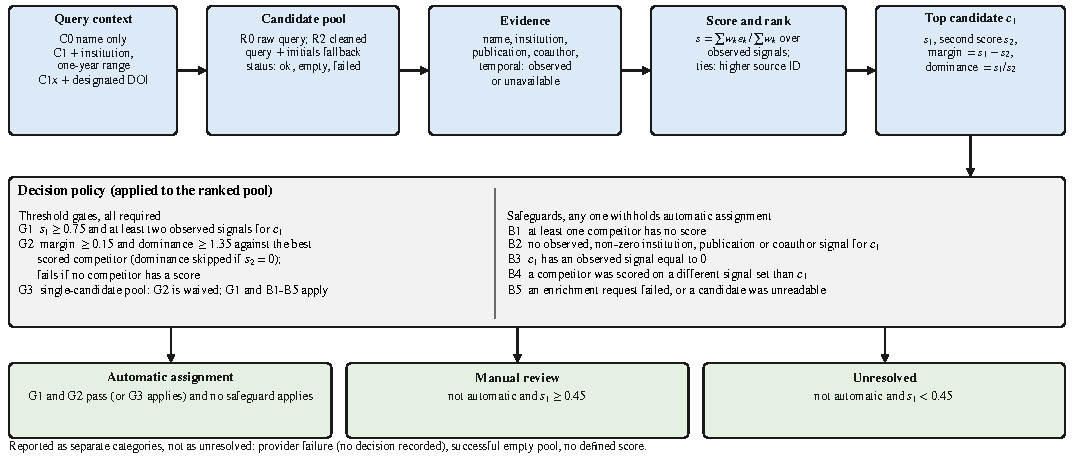
\includegraphics[width=\textwidth]{figures/methodology.pdf}
\caption{Author-resolution methodology. The decision policy (G1--G3 and B1--B5 of Table~\ref{tab:gates}) is applied to the ranked pool and yields one of three outcomes. Failed and empty pools bypass the policy. Regenerate with \texttt{figures/make\_figures.py}.}
\label{fig:methodology}
\end{figure*}

A high score is not enough for automatic assignment, for three reasons. The score is renormalized, so a score of 1.0 over a single signal is possible, and the policy requires at least two observed signals. Name agreement is common among different people, so B2 requires an observed, non-zero institution, publication or coauthor signal, and name together with temporal agreement is not sufficient. These two requirements together make automatic assignment structurally impossible when only the name is supplied: coverage is zero by design in that setting, which is a property of the policy and not evidence that the policy is safe or accurate. Third, a score can be inflated by missing evidence, and B1, B4 and B5 withhold automation when competitors were not scored comparably or evidence retrieval was incomplete. Safeguards B1 to B5 only withhold automation and route the query to manual review. None introduces a new numeric threshold, and their effect on precision and coverage has not been measured.

Three policies are applied to the same frozen pool and evidence in the experiments. The \emph{full selective policy} (artifact identifier \texttt{selective\_policy\_v2}) applies every rule of Table~\ref{tab:gates}. The \emph{threshold-gate ablation with P3 relaxation} (artifact identifier \texttt{legacy\_gates\_plus\_p3}) applies G0 to G3 and the manual-review and failure rules but not the safeguard blockers B1 to B5. It is computed offline from the same snapshot and shows what the blockers change. It is not a complete removal of equivalent protections: the margin gate G2 still requires a scored competitor, so a pool whose competitors are all unscored cannot be assigned automatically. An unscored competitor next to a scored one is, however, no longer blocked, because the margin is computed against the scored one. The \emph{forced top-one policy} (\texttt{forced\_top1}) selects $c_1$ whenever $s_1$ is defined, with no abstention. The application also attaches a High, Medium or Low display label derived from the same two score thresholds; it is a user-interface convenience, is not calibrated, and is not used in any evaluation.

Six outcome categories are kept separate in every table: automatic assignment, manual review, unresolved, successful empty retrieval, provider failure, and no candidate with a defined score. A provider failure is not an unresolved identity decision. In the application's stored status, an empty pool and a pool without a defined score both appear as unresolved with a reason, and a provider failure records no resolution; the evaluation reports each as its own category. Failure handling follows from the principle that missing evidence is not negative evidence. A candidate whose stored payload cannot be parsed is dropped from the ranking, the pool is marked incomplete, and B5 withholds automatic assignment. Enrichment failures mark the affected signal unavailable and also trigger B5.

\subsection{Context Conditions and Leakage Controls}
\label{sec:leakage}
The context $\kappa$ determines which signals can be observed. Three conditions are defined (Table~\ref{tab:conditions}). \textbf{C0} supplies the name only. \textbf{C1} adds an institution and an active-year range. In the LAGOS-AND experiment it supplies no publication identifiers, so publication overlap is excluded from the primary condition. \textbf{C1x} additionally supplies publication identifiers whose independence from the gold evidence is not established.

Every DOI used in a benchmark is registered with one of three purposes. \texttt{gold\_evidence} marks a DOI used to establish the expected identity, \texttt{query\_context} marks one chosen independently of the gold evidence and eligible for the query context, and \texttt{both} marks one that serves both roles and requires a written justification. DOIs registered as \texttt{gold\_evidence} are removed from C1. DOIs registered as \texttt{both} contribute only to C1x. Publication-overlap results that rely on a leakage-prone DOI are therefore exploratory by construction. Query contexts are derived from a frozen seed and the register and are never edited after candidates have been generated; a change creates a new dataset version. C1x is reported separately and is never mixed into the primary evaluation.

\begin{table}[t]
\caption{Context conditions. Only C1 supports primary claims.}
\label{tab:conditions}
\centering
\footnotesize
\renewcommand{\arraystretch}{1.1}
\begin{tabular}{@{}p{0.10\columnwidth}p{0.55\columnwidth}p{0.24\columnwidth}@{}}
\toprule
\textbf{Cond.} & \textbf{Context supplied} & \textbf{Status} \\
\midrule
C0 & Name only & Control; automatic coverage zero by design \\
C1 & C0 plus institution and active-year range; no publication identifiers & Primary \\
C1x & C1 plus publication identifiers not shown to be independent of gold evidence & Exploratory only \\
\bottomrule
\end{tabular}
\end{table}

Coauthor evidence has a further constraint in this study. The benchmark gives coauthors as name strings without identifiers, and names are not scored, so coauthor evidence is unavailable in every condition and the effective signal set has at most four members.

\section{Experimental Design and Evaluation Protocol}
\label{sec:design}

This section separates what has been done from what is planned. Four things have been done: the benchmark was downloaded, verified, sampled and re-verified, and its eligible frame was counted; a 50-case seed set was frozen; an operational smoke capture of OpenAlex responses was captured and replayed offline; and the tooling that will run the evaluation was implemented and validated on synthetic data. Everything else is planned: the coverage pilot, the main sample, the independent verification, the main evaluation and its analysis. Fig.~\ref{fig:pipeline} shows the workflow, and the planned stages are drawn with dashed outlines.

\begin{figure*}[t]
\centering
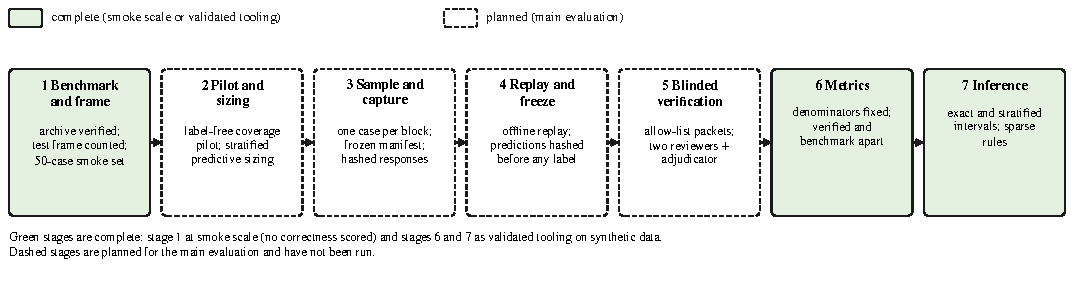
\includegraphics[width=\textwidth]{figures/evaluation_pipeline.pdf}
\caption{Experimental workflow. Completed stages ran at smoke scale only. The label audit, the evaluation and the analysis are planned. Regenerate with \texttt{figures/make\_figures.py}.}
\label{fig:pipeline}
\end{figure*}

\subsection{Benchmark}
\label{sec:benchmark}
The primary benchmark candidate is LAGOS-AND, version 2.0, released on Zenodo (DOI 10.5281/zenodo.7313353) under a CC~BY~4.0 licence~\cite{zhang2022lagosandv2}. The dataset paper and the Zenodo record describe its automatic construction from ORCID and DOI evidence~\cite{zhang2023lagosand}, and the record states that version 2.0 replaces the Microsoft Academic Graph as literature source with OpenAlex. How the ORCID attribution of each individual record was established is not described in the parts of these sources that we could read (the journal version of the dataset paper was not accessible), and we do not assume it.
We used the block-trimmed archive. Its size (743,558,936 bytes) and MD5 checksum matched the values listed by Zenodo, the compressed stream was read to its end, and we computed and recorded a SHA-256 checksum. The archive was processed by streaming. It was obtained a second time and verified again against the same size, MD5 and SHA-256 checksums, and the block catalog built from it reproduced every count in Table~\ref{tab:dataset} and the size-band counts of Section~\ref{sec:seeds}. Table~\ref{tab:dataset} gives the characteristics we measured.

\begin{table}[t]
\caption{LAGOS-AND v2.0 (block-trimmed) as measured by the preparation script.}
\label{tab:dataset}
\centering
\footnotesize
\renewcommand{\arraystretch}{1.1}
\begin{tabular}{@{}p{0.55\columnwidth}p{0.33\columnwidth}@{}}
\toprule
\textbf{Characteristic} & \textbf{Value} \\
\midrule
Data rows & 1,476,550 \\
Name blocks & 80,294 \\
(block, ORCID) identity groups & 244,564 \\
ORCIDs occurring in more than one block & 0 \\
DOIs shared by more than one ORCID & 0 \\
Publication years & 1870 to 2022 \\
Rows without an author affiliation & 14.10\% \\
Blocks eligible for sampling & 70,351 \\
\bottomrule
\end{tabular}
\end{table}

Each block collects publication records for one printed name form, and each identity group within it is defined by an ORCID value attached to its records. A complete pass over all 1,476,550 rows confirmed the publication-year range of Table~\ref{tab:dataset}; an earlier inspection of the first 16,710 rows had shown 1963 to 2022, and the 45 rows dated before 1963 lie outside that prefix. Fourteen columns are present, including the printed author name, affiliation, DOI, publication year, coauthor names and a train, test or validation flag. The \texttt{pid} column behaves like a Microsoft Academic Graph identifier and is not an OpenAlex identifier, and we do not treat it as one. Coauthors are given as name strings without identifiers, so the coauthor-ID signal cannot be observed on this dataset.

The ORCID basis of the groups creates a circularity risk. The expected identity is defined by ORCID equality, and OpenAlex candidate profiles also carry an ORCID field; the two may derive from overlapping upstream attributions. Agreement on ORCID may then reflect shared attribution and not independent verification of the person, and an error in an ORCID attribution could be present on both sides. \textbf{ORCID equality is therefore a provisional matching mechanism and not independent identity ground truth.} The ORCID field also bounds what it can label: in the smoke capture it held a value for only 57.5\% of returned candidates. These are the reasons for the independent verification of Sections~\ref{sec:labels} and~\ref{sec:audit}.

\subsection{Smoke Sample}
\label{sec:seeds}
A deterministic sampler (seed 20261119) built the 50-case smoke sample. The unit of sampling is a complete name block. Blocks with more than eight ORCID groups (2,391) and blocks in which no group has two distinct DOIs (7,552) were excluded. Eligible blocks were stratified by block size alone, using the number of unique DOIs (0--9, 10--49, 50--199 and 200 or more), ordered within each stratum by a hash of the seed and the block name, and taken round-robin only if every query-eligible group of a block fitted the target. No OpenAlex result, ORCID match or HAMMER output was used. The sample has 50 cases from 23 blocks (6, 6, 6 and 5 blocks in the four strata), with 32 train, 15 test and 3 validation cases according to the source flag. HAMMER does not train, so the flag records provenance only. Re-running the sampler on the archive reproduced every output byte for byte, apart from the recorded sampling date.

A seed contains an opaque case identifier, the printed name, an opaque group and block identifier, the context for C1 and for C1x, and sampling metadata. It contains no ORCID, no \texttt{pid} and no coauthor field. The primary C1 context is the affiliation of one designated citation of the group, normalized as described in Section~\ref{sec:affiliation}, and that citation's publication year as a one-year active range. The designated citation is the one with the smallest hash of the seed, ORCID and DOI among those that have an affiliation. Two cases have no affiliation, so their C1 context has no institution. The designated citation is a property of a group member, so it carries a weak hint of group membership. It is the kind of information a user would hold about a new paper, and we record the hint as a design limitation.

The DOI register holds 1,713 DOIs, each used by exactly one case: 1,663 registered as \texttt{gold\_evidence} (the group's other citations) and 50 as \texttt{both} (the designated citation, with a written justification). None is registered as \texttt{query\_context}, so no DOI is present in C1. The 50 designated DOIs form the C1x context. The seeds and the register were hashed and frozen before any candidate was generated.

These 50 cases are an operational pilot sample and are not the main evaluation sample. They are also not 50 independent observations, because the cases come from 23 blocks and cases within a block are related.

\subsection{Smoke Capture}
\label{sec:smoke}
The smoke capture checked whether the toolkit and the provider interface work end to end. It scored no correctness. The capture issued 92 requests, all of which returned HTTP 200: 42 author searches and 50 DOI-based works look-ups for C1x. Fifty cases need 42 and not 50 author searches because R0 and R2 issued identical primary requests in every case and therefore shared one response, ten cases repeat another case's printed name and share its request, and two initials fallbacks were issued. Every response was written to its own file and hashed before the next request. All 92 hashes verified, and the offline replay reproduced its four artifacts byte for byte across two runs. The provider-reported cost was \$0.047. An earlier attempt used a placeholder credential and received 40 HTTP 401 responses. Its records are preserved separately and are not part of the data. The capture now stops at once on HTTP 401, 403 or 429, after saving and hashing the response.

\begin{table}[t]
\caption{Smoke-capture retrieval diagnostics (50 cases, 23 blocks). The expected ORCID is the dataset's, so these counts show label availability and not identity accuracy.}
\label{tab:smoke-retrieval}
\centering
\footnotesize
\renewcommand{\arraystretch}{1.1}
\begin{tabular}{@{}p{0.60\columnwidth}p{0.10\columnwidth}p{0.10\columnwidth}@{}}
\toprule
\textbf{Diagnostic (denominator 50)} & \textbf{R0} & \textbf{R2} \\
\midrule
Expected ORCID found in the pool & 36 & 38 \\
Expected-ORCID profile ranked first & 21 & 22 \\
Expected-ORCID profile within first 5 & 32 & 34 \\
Expected ORCID absent from a successful pool & 7 & 7 \\
ORCID null in every returned candidate & 5 & 5 \\
Successful empty pool & 2 & 0 \\
Provider failure or malformed response & 0 & 0 \\
\bottomrule
\end{tabular}
\end{table}

Table~\ref{tab:smoke-retrieval} lists the retrieval diagnostics. The ORCID field was present on every returned candidate, with a value for 57.5\% of them. The two R0 pools that were empty were found by R2's initials fallback, and the other 48 pools were identical. Rank is the provider's order. These counts describe an ORCID-based diagnostic on one small sample. They do not validate identity retrieval accuracy, and they cannot support a comparison of R0 and R2, because the two shared their primary response in all 50 cases.

\begin{table}[t]
\caption{Smoke-capture replay outcomes (50 cases). No correctness is scored.}
\label{tab:smoke-replay}
\centering
\footnotesize
\renewcommand{\arraystretch}{1.1}
\begin{tabular}{@{}p{0.50\columnwidth}p{0.11\columnwidth}p{0.11\columnwidth}@{}}
\toprule
\textbf{Configuration} & \textbf{Auto} & \textbf{Manual} \\
\midrule
C0, selective\_policy\_v2 & 0 & 50 \\
C1, selective\_policy\_v2 & 4 & 46 \\
C1x (exploratory), selective\_policy\_v2 & 7 & 43 \\
\bottomrule
\end{tabular}
\end{table}

Table~\ref{tab:smoke-replay} lists the replay outcomes under the full policy; every case was either automatic or manual, and none fell into the unresolved, empty-retrieval, provider-failure or no-score categories. The zero in C0 follows from the policy under name-only evidence (Section~\ref{sec:policy}) and is not evidence of safety. C1x remains exploratory: its publication evidence comes from a DOI that is a member of the group, and publication overlap was observed for the top candidate in all 50 cases. Under the threshold-gate ablation with P3 relaxation, C1x yields 26 automatic outcomes, so the safeguard blockers withhold automation in many of the cases that would otherwise pass the threshold gates; whether this improves precision has not been measured. In C1 the institution signal was observed for the top candidate in 29 cases, the candidate had no affiliation in 19 and the query had none in 2, and the temporal signal was observed in 36 and inconclusive in 14. Signal availability, and not only the score, therefore drives the outcome. These counts do not support any claim of precision, recall or superiority over a baseline.

\subsection{Label Strategy and Verification}
\label{sec:labels}
Two kinds of label are kept apart throughout. A \emph{benchmark-derived} label is the provisional ORCID-based mapping of Section~\ref{sec:benchmark}, and it is never described as independently verified. A \emph{verified} label is reached by independent reviewers from evidence outside the benchmark labels (Section~\ref{sec:audit}). A reviewed case has one of four \emph{label states}: resolved (a definite intended person was identified), unresolved (no unique intended person exists), uncertain, or unverifiable. Every case belongs to exactly one \emph{reporting class}: Verified, Uncertain, Unverifiable or Benchmark-derived. Each class is reported with its case count, an audited case is never also Benchmark-derived, and verified and benchmark-derived observations are never combined into one accuracy figure.

The primary population is defined by one condition and policy pair: condition C1 with the full selective policy. Every automatic assignment of that pair is verified independently, and only those assignments define the primary verified precision. A pre-specified random sample of the remaining, non-automatic cases of the same pair is audited. Its frame is the entire non-automatic set, including cases in which no candidate is mapped to the expected person, so that label problems, profile fragmentation and retrieval failure are not excluded. The frame is built after capture and replay under frozen thresholds, weights, code and policy, and it uses no benchmark identity label. The sample is stratified by block size with proportional allocation (largest-remainder rounding) and drawn by a deterministic SHA-256 hash order under a predeclared seed. If strata must be merged, the rule is fixed before the draw and the original stratum sizes are still reported. The audit size is \tbd{set after the reviewer-time pilot}. When a reviewer verifies an automatic assignment, the reviewer receives the complete candidate pool, shuffled and under opaque identifiers, and cannot see HAMMER's selection, rank, score or decision.

Table~\ref{tab:scoring} states how one automatic assignment is scored against its verified label. Only uncertain and unverifiable cases leave the precision denominator. A definite identity without a matching candidate, and a case with no unique intended person, are incorrect assignments and stay in it. Uncertain and unverifiable cases remain visible and are bracketed by counting them all wrong and then all right.

\begin{table}[t]
\caption{Scoring of one automatic assignment against its verified label.}
\label{tab:scoring}
\centering
\footnotesize
\renewcommand{\arraystretch}{1.1}
\begin{tabular}{@{}p{0.50\columnwidth}p{0.20\columnwidth}p{0.13\columnwidth}@{}}
\toprule
\textbf{Verified status; selected candidate} & \textbf{Scored as} & \textbf{In denominator} \\
\midrule
Resolved; judged the same person & correct & yes \\
Resolved; judged a different person & incorrect & yes \\
Resolved; every pool candidate judged different & incorrect & yes \\
Unresolved (no unique intended person) & incorrect & yes \\
Uncertain or unverifiable, or reviewers cannot tell for the selected candidate & not scored, counted & no \\
\bottomrule
\end{tabular}
\end{table}

Benchmark-group validity and case-level candidate verification are separate questions. A reviewer first judges whether the benchmark group is \emph{pure} (all its publications belong to one person), \emph{impure} or \emph{unresolved}. A confirmed impure group is a contradiction of the benchmark label. An uncertain or unverifiable case stays outside the definite-label denominator of the audit error rate even when its group is impure; its impurity is reported separately and the uncertainty bracket is kept. A pure group whose case label is unresolved is indeterminate. For a case with a definite label, the audit error is derived from the adjudicated record and has three reasons: an impure group, a false mapping (a benchmark-mapped candidate judged a different person) and a missed mapping (an unmapped candidate judged the same person). A case counts once in the numerator and the reasons are reported separately. A cannot-tell judgment is indeterminate and never an error.

The audit error rate describes only the sampled non-automatic frame of the primary pair, and it is reported next to the benchmark-derived results of that frame. It is not used as a correction factor, and it is not applied to automatic assignments, to other conditions or policies, or to the overall retrieval results. Conditions and policies other than the primary pair (C0, C1x, the threshold-gate ablation and forced top-one) are reported as benchmark-derived. The benchmark contains only resolved identities, so false acceptance on unresolved queries is not measured, and that measure is omitted.

\subsection{Blinded Review Procedure}
\label{sec:audit}
Review has two stages. In Stage A, reviewers establish who the person is from the printed name and up to $K$ publications of the benchmark group (the designated paper always included, the others chosen and ordered by hash; $K=10$, adopted at the freeze and to be confirmed in the reviewer-time pilot), and they test the purity of the group against evidence outside the benchmark labels. No candidate profile is shown. In Stage B, reviewers judge each candidate of the shuffled pool as the same person, a different person, or undeterminable, against the Stage A identity. Every candidate must be judged before a pool can be declared to hold no matching candidate.

Packets are built by a script from an explicit allow-list of fields and are never edited by hand. The captured provider objects carry the ORCID in several fields (\texttt{orcid}, \texttt{ids.orcid} and an observed-ORCID list), and also identifiers, profile URLs and a relevance score that reveals the provider's rank, so a deny-list would fail silently when the provider adds a field. Stage B packets therefore hold only name variants, affiliation names with years, topics, a works count and yearly counts, and a capped works list from a separate, hashed capture of each candidate's works. Candidates are shuffled by a hash-seeded order that does not depend on the provider's or HAMMER's rank and carry opaque identifiers; the crosswalk to provider identifiers and the flag that says whether a case was automatic or audited are kept in a separate protected location. Automatic and audited cases are presented in the same form and in a mixed queue, so nothing shows a case's origin. Before release a packet is scanned for any ORCID-shaped string, ORCID URL, OpenAlex identifier or URL, rank or score field and HAMMER term, and for any known benchmark value. A packet is released only on zero findings, and its hash is stored with the scan report. Reviewers are asked not to use an ORCID as evidence and to record whether they met one, and results are reported separately for cases in which they did. Residual leakage through a reviewer's own searches cannot be excluded.

Two reviewers judge each case independently. A third person, who is neither a reviewer nor the person who builds the packets, adjudicates disagreements; the final label is recorded with a rationale and never overwrites the reviewers' own rows. Agreement is reported as raw agreement and Cohen's kappa~\cite{cohen1960kappa} together with the counts, because kappa is unstable at small numbers and when one category dominates. Reviewers are outside the project team and have not seen HAMMER outputs or the benchmark ORCID labels for the audited cases; their number, hours and arrangements are \tbd{stated at freeze}. The measured reviewer time of a small pilot on smoke cases sets the audit size.

\subsection{Sampling Design}
\label{sec:sampling}
The main evaluation uses new cases. Its frame is the set of eligible blocks of the test split (Table~\ref{tab:frame}), excluding the 23 smoke blocks and the blocks reserved for the coverage pilot. The study therefore concerns a restricted, benchmark-defined population of ambiguous author blocks (at least two and at most eight ORCID groups); it does not establish performance across all author names or on the most ambiguous names that the cap excludes. Blocks are stratified by the fixed size bands of Section~\ref{sec:seeds}.

\begin{table}[t]
\caption{Eligible blocks of the test split after excluding the 23 smoke blocks, counted from the verified archive. The coverage pilot removes further blocks before the main draw.}
\label{tab:frame}
\centering
\footnotesize
\renewcommand{\arraystretch}{1.1}
\begin{tabular}{@{}lrr@{}}
\toprule
\textbf{Band} & \textbf{Unique DOIs} & \textbf{Eligible blocks} \\
\midrule
S & 0--9 & 8,038 \\
M & 10--49 & 8,360 \\
L & 50--199 & 1,173 \\
XL & 200 or more & 9 \\
\midrule
All & & 17,580 \\
\bottomrule
\end{tabular}
\end{table}

The primary sample takes one case per block: the case-eligible group with the smallest SHA-256 of the seed, block and ORCID. The other case-eligible groups of a drawn block are recorded as secondary cases, are benchmark-derived only, and are used only in an exploratory block-clustered sensitivity analysis. Each ORCID occurs in exactly one block, so one case per block is also one case per person. Within a stratum, blocks are drawn in SHA-256 order of the seed, role and block, which is equivalent to simple random sampling without replacement. Let $N_h$ be the number of eligible blocks in stratum $h$, $n_h$ the number sampled and $g_i$ the number of case-eligible groups in the block of case $i$. A case is included with probability $(n_h/N_h)/g_i$, so the block-level estimand E1 (a random eligible block, then a random eligible person in it) uses the weight $N_h/n_h$, and the person-level estimand E2 uses $(N_h/n_h)\,g_i$~\cite{horvitz1952}. E1 is primary and E2 is secondary, and the two are never conflated.

The allocation across strata is proportional with per-stratum floors. A floor at or above the size of a stratum takes the whole stratum (a census), the remainder is allocated to the unbound strata proportionally to their sizes, and rounding follows the largest-remainder rule. The floors are 0 for strata S, M and L and 9 for stratum XL, which makes XL a census of its nine eligible blocks. Seeds are derived and not chosen: the seed of each role (pilot, main, audit, packet order) is the first eight hexadecimal digits of the SHA-256 of the string \texttt{HAMMER|}\textit{role}\texttt{|}\textit{freeze identifier}, read as an integer, so that no favourable seed can be selected. The total $N$ follows from the pilot (Section~\ref{sec:pilot}). The smoke, pilot and main samples are drawn by separate hash roles and are disjoint. Each draw writes a manifest that holds no ORCID, records the inclusion probabilities as exact fractions and is bound to a SHA-256 of its content and of the selector's source. The mapping from opaque case identifiers to benchmark ORCIDs is held separately.

\subsection{Coverage Pilot and Sample Size}
\label{sec:pilot}
The precision of the verified result depends on the number of automatic assignments, which is random. The share of automatic assignments (coverage) is estimated first by a label-free pilot: a sample of blocks from the test frame, drawn by the same rule with a separate seed and removed from the main frame, is captured and replayed under frozen thresholds, weights, code and policy. The pilot scores no correctness and uses no label, only each case's decision category.

Let $a_h$ be the automatic assignments among $n_{p,h}$ pilot cases of stratum $h$. Coverage $c_h$ is given the prior Beta$(\alpha_0,\beta_0)$, with the Jeffreys prior $(\tfrac12,\tfrac12)$~\cite{jeffreys1946} as the primary choice and the uniform prior as a sensitivity analysis, so $c_h\mid\text{pilot}\sim\text{Beta}(\alpha_0+a_h,\beta_0+n_{p,h}-a_h)$; a stratum without pilot data keeps the prior. For a total sample size $N$, the allocation above gives $n_h(N)$, and the automatic count of stratum $h$ is beta-binomial with parameters $n_h(N)$ and the posterior of $c_h$. The strata are independent, so the distribution of the total $A=\sum_h A_h$ is obtained by exact convolution. The sample size is the smallest $N$ with
\[
\Pr(A\ge m')\ \ge\ 1-\beta
\]
that also holds for every $N'$ up to a declared $N_{\max}$, which guards against non-monotone behaviour of the allocation: largest-remainder rounding can reduce a stratum's share when $N$ grows. The probability $\beta$ is 0.05, the level $\gamma$ is 0.10, $N_{\max}$ is 2,500, and the pilot takes 100, 100 and 50 blocks from the S, M and L strata and none from XL, because all nine XL blocks are needed for the census. Smaller pilots (30 to 40 cases per stratum) left the predictive rule about two percentage points under its target when the prior was mismatched, and $\beta=0.05$ costs about 6 to 7\% more cases than $\beta=0.10$ (Section~\ref{sec:validation}). The target number of automatic assignments $m'$ depends on reviewer capacity, which is not yet known; it is \tbd{fixed after the reviewer-time pilot}, and the main sample size is therefore reported conditionally on $m'$ until then. As a sensitivity check, each $c_h$ is replaced by its exact one-sided Clopper--Pearson lower limit~\cite{clopper1934} at level $1-\gamma/H$ over the $H$ strata (zero without pilot data), and both sample sizes are reported. The rule $N=\lceil m'/c\rceil$ is not used, because it reaches $m'$ only about half the time. The sample size is fixed before the main capture and is not extended after results are seen.

\subsection{Evaluation Metrics}
\label{sec:metrics}
Table~\ref{tab:metrics} defines the measures, their label basis and their denominators. Every drawn primary case stays in the case accounting and falls into exactly one of six outcome categories: automatic, manual, unresolved, successful empty retrieval, provider failure, or no defined score. A case need not be in every denominator. Let $N$ be the number of primary cases. All benchmark labels are resolved, so the \emph{candidate-pool mapping rate} is the share of the $N$ cases whose expected person has a mapped profile in the captured R2 pool; it does not measure the provider's catalog, since a failed search does not show that the person is absent from OpenAlex. R2 is the primary pool for every retrieval measure, and R0 remains a descriptive comparison. \emph{End-to-end} success@$k$ and MRR use all $N$ cases (a failure or an empty pool counts as a miss), whereas \emph{conditional} Recall@$k$ and MRR use only the cases with a mapped profile. The conditional measure alone would let a retriever look effective by excluding the cases in which it retrieved nothing, so the two are always shown together. Overall retrieval is benchmark-derived, keeps all $N$ cases, and is never adjusted by any audit or verified result. Verified retrieval is reported separately, for the automatic assignments and for the audit sample, using only cases with a definite verified label; excluded categories (not yet verified, uncertain, unverifiable, ground-truth unresolved, incomplete judgments) are counted separately, and a HAMMER abstention never removes an otherwise adjudicable case. Its conditional measures use the cases with a verified-same candidate in the pool as denominator, and every other judgment category is reported separately.

\begin{table*}[t]
\caption{Measures, label basis and denominators ($N$ primary cases). Every rate is reported with its numerator and denominator.}
\label{tab:metrics}
\centering
\footnotesize
\renewcommand{\arraystretch}{1.12}
\begin{tabular}{@{}p{0.20\textwidth}p{0.12\textwidth}p{0.34\textwidth}p{0.24\textwidth}@{}}
\toprule
\textbf{Measure} & \textbf{Label basis} & \textbf{Numerator} & \textbf{Denominator} \\
\midrule
Automatic, manual, unresolved, empty, failure and no-score rates & label-free & Cases in the category & All $N$ cases \\
Candidate-pool mapping rate & benchmark & Cases with a mapped profile in the R2 pool & All $N$ cases \\
End-to-end success@$k$, $k\in\{1,5,10\}$; end-to-end MRR & benchmark & Mapped within the first $k$ provider-ordered candidates; reciprocal rank, unmapped counts as 0 & All $N$ cases \\
Conditional Recall@$k$; conditional MRR & benchmark & First mapped profile within $k$; reciprocal rank & Cases with a mapped profile \\
Automatic precision; selective risk & verified & Automatic assignments scored correct (Table~\ref{tab:scoring}); incorrect & Automatic assignments scored correct or incorrect \\
Audit label-error rate & verified & Audited cases with a definite label whose adjudicated record contradicts the benchmark & Audited non-automatic cases with a definite label \\
Verified retrieval, by subset & verified & As for overall retrieval, on verified cases & Cases with a definite verified label, by subset \\
\bottomrule
\end{tabular}
\end{table*}

Precision and coverage are always reported together. When a denominator is zero the measure is reported as undefined and never as zero, and precision is undefined when there are no automatic assignments. The six outcome categories are kept separate in every results table. Retrieval failure, absence of the expected person from the pool and an undecided case are likewise separate. Recall, success and MRR use the provider's order and not HAMMER's score. The coverage and verified precision of other conditions and policies would need their own verification design; they are reported as benchmark-derived.

\subsection{Statistical Inference}
\label{sec:inference}
Strata are finite populations sampled without replacement, so a binomial interval is a model and not the design, and no interval is called design-exact. Three regimes are used. (R1) Per stratum, a Clopper--Pearson interval on the stratum count is reported as a conservative superpopulation approximation; the sampling fraction of each stratum is reported, and a stratum that is a census gets no interval. (R2) The frame-weighted pooled estimate for E1 (and E2) is given with a stratified percentile bootstrap~\cite{efron1979bootstrap} that resamples cases within strata and holds census strata fixed. (R3) Sparse automatic precision is reported as counts with exact intervals, and when there are no errors with the one-sided upper bound $1-0.05^{1/n}$; no bootstrap is used, and a bootstrap on zero errors is never reported. A stratum too small to resample is reported without an interval. The pooled interval is then withheld unless a negligible-weight rule, fixed before the draw, drops that stratum from the pooled estimand, in which case the estimand is relabelled. The numerical warning thresholds (the sampling fraction that flags a stratum, the sparse-count limits, the minimum stratum size for the bootstrap and the contributing-block warning of the clustered analysis) are fixed at the freeze: the sampling fraction that flags a stratum is 0.10, the sparse-count warnings are 30 automatic assignments and 5 errors, the minimum stratum size for the bootstrap is 20 non-census cases, the clustered-analysis warning is 20 contributing blocks, and a stratum with a frame weight below 0.005 is dropped from the pooled estimand and reported separately (this affects only XL, at 0.05\% of the frame). They are diagnostics and not validity boundaries. Paired comparisons between conditions and policies are descriptive and benchmark-derived. A block-clustered bootstrap with a leave-one-block-out check is an exploratory sensitivity analysis on the secondary cases only and is never merged with the primary estimates.

\subsection{Validation of the Evaluation Tooling}
\label{sec:validation}
The evaluation tooling was tested before any evaluation data existed, so that a defect in the tooling cannot be mistaken for a property of HAMMER. The metrics, the sample-size procedure, the selector, the evaluation-freeze manifest, the capture stop-condition guard, the packet builder with its leak scan, the candidate-works capture and release driver, the review-record layer, the report assembly and the table generator were each checked on synthetic data against references that do not share their code: hand-computed values, exact rational arithmetic and independent simulation. In each case, deliberate defects were injected into the code one at a time to confirm that the tests detect them. A synthetic end-to-end rehearsal with a known hidden truth reproduced the verified precision and the audit error rate exactly. On the 50 smoke cases the metrics agreed with an independent diagnostic case by case, and the allow-listed packets built in memory from the 306 captured candidate profiles contained no benchmark ORCID although the raw provider objects did.

Repeated-sampling simulations on a synthetic population were used to check the statistical procedures. The E1 and E2 estimators were unbiased for their own estimands, and applying block-level weights to the person-level target was biased by about twenty standard errors. Per-stratum Clopper--Pearson intervals covered 0.96 to 0.97 at the nominal 0.95. The pooled stratified bootstrap covered 0.935, slightly below nominal. The predictive sample-size rule reached its 0.90 target (0.899) when the true coverage was drawn from its prior, but only 0.88 when the true coverage distribution was narrower than the prior and the pilot was small, whereas the lower-bound check was conservative (0.998) and the rule $N=\lceil m'/c\rceil$ reached 0.55 to 0.68. These are properties of the procedures on synthetic data and not results about HAMMER. They are why per-stratum Clopper--Pearson intervals are reported next to pooled bootstrap intervals, why both sample sizes are reported, and why the size of the pilot matters.

\subsection{Affiliation Cleaning}
\label{sec:affiliation}
Affiliations in the benchmark contain source markers. The seed builder replaces the tab marker \texttt{\#TAB\#} with a space and collapses whitespace, and it keeps the original string in a separate file. Other markers, \texttt{\#R\#\#N\#} and \texttt{\#N\#}, were observed in the sample and are not handled, and some strings contain long multi-institution text. Extending the rule would change the frozen seed and would therefore define a new dataset version. Whether and how to extend it is undecided. The requirements are that the raw affiliation is always preserved, that every transformation is documented, and that the normalizer is separately versioned. No cleaning beyond the tab marker has been done.

\subsection{Status of the Main Evaluation}
\label{sec:main}
The main evaluation has not been run, and no result of it is reported. The protocol above is fixed, and the tooling that executes it has been validated on synthetic data. An evaluation freeze (a manifest of file hashes, the effective configuration, the parameters above and the derived seeds, written before any provider request) and a coverage-pilot draw of 250 blocks have been completed; the pilot leaves 7,938, 8,260, 1,123 and 9 eligible blocks in the S, M, L and XL strata for the main draw. Four freezes (F1 to F4) were written, and the first three were superseded before any usable data existed because the frozen file set had to change: the stop-condition guard was added (F1 to F2), the seed-freeze file written for the capture inputs lacked fields that the capture step verifies (F2 to F3), and the guard mis-handled compressed responses (F3 to F4). The last two defects were found by the first real capture attempts, were fixed with regression tests, and the failed attempts are kept as negative results. The coverage pilot has not been captured and the main sample has not been drawn, because a credential for the provider was not supplied and no money was to be spent. The stop conditions of the capture are: HTTP 401, 403 or 429, an exhausted request budget, three consecutive server errors or transport errors, and 80\% of a cost ceiling. What was captured instead, within the free keyless tier of the provider, is an \emph{exploratory} sample of 50 blocks drawn from the main frame with the derived main seed (disjoint from the smoke and pilot blocks), of which 18 cases were completed before the shared free daily budget ended (Section~\ref{sec:res-samples}). Because that draw consumed the derived main seed, any confirmatory main sample needs a new freeze identifier and must also exclude these blocks. The exploratory results are benchmark-derived and are never used to tune a parameter or to size the confirmatory sample. Still open are the coverage pilot, $m'$ and the resulting $N$, the audit size and merging rule, the confirmatory capture, and the reviewer arrangements, which are not simulated. No setting is tuned on the results of the main evaluation, and a changed protocol is a new version that needs an independent evaluation. The main sample consists of new cases and does not reuse the smoke cases for confirmatory claims. The smoke sample has 50 cases from 23 blocks, which are clustered observations and not 50 independent ones, and no interval is reported for it.

\section{Results}
\label{sec:results}
No independently verified result exists. The blinded review that the protocol requires has not been performed, and the main evaluation of Section~\ref{sec:design} has not been run. This section reports what was obtained instead, each part labelled by its basis. Subsections~\ref{sec:res-samples} to~\ref{sec:res-planning} are \emph{exploratory and benchmark-derived}: they come from the offline replay of two small real samples, and ``agreement with the benchmark'' means agreement with the provisional ORCID label of Section~\ref{sec:benchmark}, not identity accuracy. No figure here is pooled with another, corrected by an audit, or called precision of the system. Subsection~\ref{sec:res-pending} lists the protocol results that are not reported.

\subsection{Samples and Scope}
\label{sec:res-samples}
\textbf{Smoke sample.} 50 cases from 23 blocks, captured with 92 hashed responses (Section~\ref{sec:smoke}). It is not a probability sample, and its cases are related within blocks. We therefore give every figure for the 50 cases and, for the selective results, also for one case per block (23 cases).

\textbf{Exploratory sample.} A second sample of 50 blocks, one primary case each, was drawn from the main frame with the derived main seed of freeze F4 (strata S, M and L with 23, 24 and 3 cases), disjoint from the smoke blocks and the 250 pilot blocks. No credential was available and no money was to be spent, so the capture used OpenAlex's free keyless tier, with the stop guard of Section~\ref{sec:main} set to a cost ceiling of USD 0.10. After 38 successful requests the provider answered HTTP 429, because the shared free daily budget was exhausted, and the capture stopped after the 18th case (nine S and nine M cases from 18 different blocks). The cases are processed in the order of their opaque identifiers, which is unrelated to the strata, so these 18 are a random subset of the drawn 50; they are reported as an \emph{18-case exploratory sample} with no inference to the frame. An earlier attempt on this sample sent 70 requests that were all recorded as decoding errors because of a defect in the stop guard (it re-wrapped an already decoded body with the wire response's compression header, which mock transports without compression could not show); that run produced no usable data, was kept as a negative result, and the defect was fixed with a regression test. Intervals below are exact Clopper--Pearson intervals that treat cases as independent; for the smoke sample they are optimistic because of clustering.

\subsection{Outcome Categories}
\label{sec:res-outcomes}
% generated by scripts/analyze_free_evaluation.py (T019); do not edit by hand
\begin{table*}[t]
\caption{Outcome categories of the offline replay under each condition and policy (benchmark-independent counts). Smoke: 50 cases from 23 blocks. Exploratory: 18 complete cases from 18 blocks. Auto = automatic, Man = manual review, Unres = unresolved, Empty = successful empty pool, Fail = provider failure, NoSc = no defined score.}
\label{tab:exp-outcomes}
\centering
\footnotesize
\begin{tabular}{@{}llrrrrrrrrrrrr@{}}
\toprule
 & & \multicolumn{6}{c}{Smoke (50)} & \multicolumn{6}{c}{Exploratory (18)} \\
\cmidrule(lr){3-8}\cmidrule(lr){9-14}
Cond. & Policy & Auto & Man & Unres & Empty & Fail & NoSc & Auto & Man & Unres & Empty & Fail & NoSc \\
\midrule
C0 & selective & 0 & 50 & 0 & 0 & 0 & 0 & 0 & 18 & 0 & 0 & 0 & 0 \\
C0 & gates+P3 & 0 & 50 & 0 & 0 & 0 & 0 & 0 & 18 & 0 & 0 & 0 & 0 \\
C0 & forced top-1 & 50 & 0 & 0 & 0 & 0 & 0 & 18 & 0 & 0 & 0 & 0 & 0 \\
C1 & selective & 4 & 46 & 0 & 0 & 0 & 0 & 0 & 18 & 0 & 0 & 0 & 0 \\
C1 & gates+P3 & 4 & 46 & 0 & 0 & 0 & 0 & 0 & 18 & 0 & 0 & 0 & 0 \\
C1 & forced top-1 & 50 & 0 & 0 & 0 & 0 & 0 & 18 & 0 & 0 & 0 & 0 & 0 \\
C1x & selective & 7 & 43 & 0 & 0 & 0 & 0 & 3 & 15 & 0 & 0 & 0 & 0 \\
C1x & gates+P3 & 26 & 24 & 0 & 0 & 0 & 0 & 8 & 10 & 0 & 0 & 0 & 0 \\
C1x & forced top-1 & 50 & 0 & 0 & 0 & 0 & 0 & 18 & 0 & 0 & 0 & 0 & 0 \\
\bottomrule
\end{tabular}
\end{table*}

Table~\ref{tab:exp-outcomes} counts the six outcome categories under every condition and policy. In every configuration and both samples each case was either automatic or manual: there was no unresolved, empty-pool, provider-failure or no-score outcome. Under C0 (name only) no case was assigned automatically by either policy with safeguards or by the threshold gates, as the policy guarantees by construction. Under the primary condition C1 with the full selective policy, 4 of the 50 smoke cases (8\%, 95\% CI 2--19\%) and 0 of the 18 exploratory cases (upper limit 19\%) were assigned automatically. The threshold-gate ablation gave the same counts under C1 (4 and 0), so the safeguards B1 to B5 changed no outcome under C1 in these samples. Under the exploratory condition C1x, whose publication evidence comes from a member of the identity group and is therefore leakage-prone, the full policy assigned 7 of 50 and 3 of 18 cases, while the ablation without the safeguards assigned 26 of 50 and 8 of 18: the safeguards withheld automation in 19 and 5 cases respectively.

\subsection{Candidate Retrieval}
\label{sec:res-retrieval}
% generated by scripts/analyze_free_evaluation.py (T019); do not edit by hand
\begin{table*}[t]
\caption{Benchmark-derived retrieval diagnostics (provisional ORCID agreement, not identity accuracy). The pool is the captured R2 pool; R0 is descriptive and shares its response with R2 whenever the requests are identical. Rank is the provider's order. Intervals are Clopper--Pearson and ignore clustering of cases within blocks.}
\label{tab:exp-retrieval}
\centering
\footnotesize
\begin{tabular}{@{}lrrrr@{}}
\toprule
 & \multicolumn{2}{c}{Smoke (50)} & \multicolumn{2}{c}{Explor.\ (18)} \\
\cmidrule(lr){2-3}\cmidrule(lr){4-5}
Measure (R2 pool) & Count & 95\% CI & Count & 95\% CI \\
\midrule
Expected ORCID in pool & 38/50 & [0.62, 0.87] & 13/18 & [0.47, 0.90] \\
Success@1 (end to end) & 22/50 & [0.30, 0.59] & 7/18 & [0.17, 0.64] \\
Success@5 & 34/50 & [0.53, 0.80] & 12/18 & [0.41, 0.87] \\
Success@10 & 38/50 & [0.62, 0.87] & 13/18 & [0.47, 0.90] \\
Conditional Recall@1 & 22/38 & [0.41, 0.74] & 7/13 & [0.25, 0.81] \\
R0: expected ORCID in pool & 36/50 & [0.58, 0.84] & 12/18 & [0.41, 0.87] \\
\bottomrule
\end{tabular}
\end{table*}

Table~\ref{tab:exp-retrieval} gives the retrieval diagnostics. The R2 pool never failed and was never empty, with a mean of 6.1 candidates in the smoke sample and 8.6 in the exploratory sample (at most ten in both). The profile carrying the benchmark ORCID was in the pool for 38 of 50 smoke cases (76\%, CI 62--87\%) and for 13 of 18 exploratory cases (72\%, CI 47--90\%); it was the provider's first candidate in 22 of 50 (44\%) and in 7 of 18 (39\%), and within the first five in 34 of 50 and 12 of 18. Among the cases whose pool contained it, the provider ranked it first in 22 of 38 and 7 of 13. The end-to-end mean reciprocal rank was 0.54 and 0.50. R0 and R2 differed little: R0 found the profile in 36 of 50 and 12 of 18 cases, and the only difference was that R0 returned an empty pool in 2 and 1 cases, which R2's initials fallback filled. Since the two share their primary response whenever the requests are identical, no comparison of the two strategies is made. For 12 of 50 and 5 of 18 cases the expected ORCID was absent from a successful pool. These counts include cases in which the right person's profile carries no ORCID, which the diagnostic cannot see, so they bound label availability and not retrieval accuracy.

\subsection{Selective Resolution (Benchmark-Derived)}
\label{sec:res-selective}
% generated by scripts/analyze_free_evaluation.py (T019); do not edit by hand
\begin{table*}[t]
\caption{Benchmark-derived selective results. Coverage is the share of cases assigned automatically; precision is the share of automatic assignments whose selected profile carries the benchmark ORCID (provisional, never independent verification). Forced top-1 never abstains, so its precision is a top-1 agreement rate. With zero errors in $n$ automatic assignments the one-sided 95\% upper bound on the error rate is $1-0.05^{1/n}$.}
\label{tab:exp-selective}
\centering
\footnotesize
\begin{tabular}{@{}llrrrr@{}}
\toprule
Dataset & Cond. / policy & Automatic & Coverage (95\% CI) & Agree with benchmark & Precision (95\% CI) \\
\midrule
Smoke, 50 cases & C1, selective & 4 & 8\% [0.02, 0.19] & 3 & 75\% [0.19, 0.99] \\
Smoke, 50 cases & C1, gates+P3 & 4 & 8\% [0.02, 0.19] & 3 & 75\% [0.19, 0.99] \\
Smoke, 50 cases & C1, forced top-1 & 50 & 100\% [0.93, 1.00] & 17 & 34\% [0.21, 0.49] \\
Smoke, 50 cases & C1x, selective & 7 & 14\% [0.06, 0.27] & 7 & 100\% [0.59, 1.00] \\
Smoke, 50 cases & C1x, gates+P3 & 26 & 52\% [0.37, 0.66] & 25 & 96\% [0.80, 1.00] \\
\midrule
Smoke, 23 blocks & C1, selective & 2 & 9\% [0.01, 0.28] & 2 & 100\% [0.16, 1.00] \\
Smoke, 23 blocks & C1, gates+P3 & 2 & 9\% [0.01, 0.28] & 2 & 100\% [0.16, 1.00] \\
Smoke, 23 blocks & C1, forced top-1 & 23 & 100\% [0.85, 1.00] & 8 & 35\% [0.16, 0.57] \\
Smoke, 23 blocks & C1x, selective & 4 & 17\% [0.05, 0.39] & 4 & 100\% [0.40, 1.00] \\
Smoke, 23 blocks & C1x, gates+P3 & 12 & 52\% [0.31, 0.73] & 11 & 92\% [0.62, 1.00] \\
\midrule
Exploratory, 18 & C1, selective & 0 & 0\% [0.00, 0.19] & 0 & undefined \\
Exploratory, 18 & C1, gates+P3 & 0 & 0\% [0.00, 0.19] & 0 & undefined \\
Exploratory, 18 & C1, forced top-1 & 18 & 100\% [0.81, 1.00] & 6 & 33\% [0.13, 0.59] \\
Exploratory, 18 & C1x, selective & 3 & 17\% [0.04, 0.41] & 3 & 100\% [0.29, 1.00] \\
Exploratory, 18 & C1x, gates+P3 & 8 & 44\% [0.22, 0.69] & 7 & 88\% [0.47, 1.00] \\
\bottomrule
\end{tabular}
\end{table*}

Table~\ref{tab:exp-selective} gives coverage and benchmark agreement. Under C1 with the full policy, 3 of the 4 automatic smoke assignments carried the benchmark ORCID (75\%, exact CI 19--99\%), and 2 of 2 in the one-case-per-block view; the exploratory sample had no automatic assignment, so no precision is defined. The one disagreeing smoke assignment cannot be classified without verification: it may be a wrong assignment or a benchmark labelling problem. Under C1x the automatic assignments agreed with the benchmark in 7 of 7 and 3 of 3 cases under the full policy, but C1x is exploratory and leakage-prone. The forced top-one policy, which never abstains and uses HAMMER's score ranking, agreed with the benchmark for 17 of 50 smoke cases (34\%) and 6 of 18 exploratory cases (33\%) under C1, whereas the provider's own first candidate agreed for 22 of 50 and 7 of 18. HAMMER's heuristic ordering of the pool therefore did not improve on the provider's order in these samples.

\subsection{Why Coverage Is Low: Gate Failures}
\label{sec:res-gates}
Of the 68 cases, all had a candidate pool under C1, and the top candidate's score was high: the median was 0.88 in both samples and only one case had a score below the automatic threshold of 0.75. The binding conditions were competition and evidence. Among the 50 smoke cases, 37 had a margin below 0.15 against a scored competitor, 44 a dominance ratio below 1.35, and 14 fewer than two observed signals for the top candidate; among the 18 exploratory cases the counts were 14, 17 and 3 (the conditions overlap). The institution signal was observed for the top candidate in 29 of 50 and 11 of 18 cases, and candidates of one pool were scored over different signal sets in 36 of 50 and 10 of 18 cases, the situation that safeguard B4 treats. In short, a high score is common, but it is rarely separated from the scores of similarly named competitors.

\subsection{Planning the Verified Evaluation}
\label{sec:res-planning}
% generated by scripts/analyze_free_evaluation.py (T019); do not edit by hand
\begin{table}[t]
\caption{Main-sample size $N$ needed for at least $m'$ automatic assignments with probability 0.95, by the stratified predictive rule, under \emph{assumed} pilot outcomes (coverage $c$ in every stratum, pilot of 100, 100 and 50 cases; frame 7,938, 8,260, 1,123 and 9 blocks, XL a census). This is a planning illustration and not data.}
\label{tab:exp-planning}
\centering
\footnotesize
\begin{tabular}{@{}rrrrr@{}}
\toprule
$c$ & $m'$ & $N$ (Jeffreys) & $N$ (uniform) & $N$ (lower bound) \\
\midrule
0.05 & 16 & 465 & 411 & 1478 \\
0.05 & 32 & 951 & 850 & $>$2500 \\
0.05 & 100 & $>$2500 & $>$2500 & $>$2500 \\
0.10 & 16 & 221 & 206 & 487 \\
0.10 & 32 & 435 & 412 & 876 \\
0.10 & 100 & 1359 & 1294 & 2439 \\
0.20 & 16 & 110 & 106 & 190 \\
0.20 & 32 & 209 & 203 & 339 \\
0.20 & 100 & 630 & 618 & 937 \\
\bottomrule
\end{tabular}
\end{table}

The label-free automatic rate under C1 was 4 of 68 cases (6\%) across both samples, which are not a probability sample, so we use it only to pick a planning range. Table~\ref{tab:exp-planning} shows the main-sample size that the stratified predictive rule would need under assumed pilot outcomes. For a target of $m'=32$ automatic assignments, about 435 primary cases are needed at a coverage of 0.10 and about 950 at 0.05, and a target of 100 assignments is out of reach within $N_{\max}=2{,}500$ at 0.05. A verified evaluation at the observed coverage would therefore have to review every one of its roughly 30 automatic assignments and also audit a sample of several hundred cases, which is a reviewer workload the project has not yet arranged.

\subsection{Protocol Results Not Reported}
\label{sec:res-pending}
The protocol of Section~\ref{sec:design} yields four results that need the label-free coverage pilot, the main sample and independent reviewers: a case-accounting table for the frozen main evaluation, the independently verified precision of automatic assignments, the audit of benchmark labels, and reviewer agreement. None of these has been run, so none is reported here, and the benchmark-derived observations above must not be read as substitutes for them. Independent verification, confirmatory sampling and reviewer-agreement analysis are left to future work, and no independently verified automatic precision or reviewer-agreement estimate is claimed in this study.

\section{Discussion}
\label{sec:discussion}
The observations of Section~\ref{sec:results} come from 68 real queries, are benchmark-derived and are partly clustered. We use them to say where the design is limited, and not to estimate how accurate it is.

\textbf{Coverage is limited by competition, not by weak evidence.} The top candidate's score was high in almost every case (median 0.88), yet only 4 of 50 smoke queries and none of 18 exploratory queries were assigned automatically under C1. The reason is visible in the gate counts: a margin below 0.15 or a dominance ratio below 1.35 in the large majority of cases (37 and 44 of 50), and fewer than two observed signals in 14 of 50. In a block of same-name authors, several candidates share the printed name and often a topic and affiliation, so each scores close to the others. A fixed-weight score over name, institution and years separates people poorly when the name signal, which carries the largest weight, is saturated for all of them. Raising coverage by lowering the margin or dominance thresholds would convert exactly these cases into automatic assignments of a candidate that is barely distinguished from its competitor, so the low coverage is the policy doing what it was designed to do. Whether it does so at the right price is the question the verified evaluation must answer.

\textbf{The heuristic ordering did not beat the provider's order.} Under C1 the top candidate by HAMMER's score agreed with the benchmark label in 34\% and 33\% of the queries, whereas the provider's first candidate agreed in 44\% and 39\%. With so few cases the difference is not established, but it removes any basis for claiming that the five-signal score improves ranking, and it suggests that candidates are being reordered mostly by name similarity, which the provider has already used. We do not know how far this reflects the weights, the missing coauthor signal on this benchmark, or the limited context supplied; the weights were never tuned and the score is not a probability.

\textbf{Retrieval is a ceiling.} The profile carrying the benchmark ORCID was missing from the pool for about a quarter of the queries (12 of 50, 5 of 18), and no ranking or decision rule can recover it. Some of these are retrieval failures, for example profiles split across several identifiers or a name form that the provider's search does not match, and some are label artefacts, such as a right-person profile without an ORCID. Telling them apart needs the independent review, which is why the design reports retrieval and assignment separately and keeps the verified retrieval measures apart from the benchmark-derived ones.

\textbf{The safeguards matter where evidence is cheap.} Under C1 the safeguards B1 to B5 changed no outcome, but under the leakage-prone C1x they withheld automation in 19 of 26 smoke cases and 5 of 8 exploratory cases. This is consistent with their purpose, since publication overlap with a group member's own paper is an easy and unreliable signal, but whether the withheld cases were wrong is unknown. We do not claim that the safeguards improve precision.

\textbf{What the label cannot say.} One of the four automatic smoke assignments disagreed with the benchmark. It may be an error of the system or of the label, and only independent review can decide. This single case shows why the design verifies every automatic assignment, and why the benchmark agreement reported here is not called precision.

\textbf{Consequences for a verified evaluation.} At the observed automatic rate of about 6\% a verified evaluation targeting 32 automatic assignments needs several hundred to about a thousand primary cases (Table~\ref{tab:exp-planning}), and reviewers would have to judge every automatic assignment and an audit sample. The cost of verification therefore scales with the coverage, which is itself small. Raising coverage in a defensible way, for example by supplying richer context or by resolving institutions to identifiers before scoring, would reduce the review burden before it improves any precision figure.

\textbf{Limits of these observations.} The samples are small (68 queries), the smoke sample is clustered into 23 blocks, the exploratory sample is a random subset of a stratified draw with no L or XL case, the label is provisional, a single provider and date are involved, and several comparisons rest on one to four cases. They are hypotheses about the behaviour of the approach, to be confirmed or rejected by the planned evaluation.

% PROPOSED replacement for sections/08_threats_limitations.tex. NOT APPLIED. States only limitations that hold regardless of the results.
\section{Threats to Validity and Limitations}
\label{sec:threats}
\textbf{Label validity.} The expected identity is derived from ORCID values, and OpenAlex profiles may carry ORCID values from overlapping upstream sources, so agreement with the benchmark is not independent verification. Independent verification covers every automatic assignment of the primary pair and an audit sample of its non-automatic cases. Results for the other cases, and all results for other conditions and policies, rest on benchmark-derived labels. The audited error rate describes only the sampled frame, is reported but not used for correction, and is not transferable. Uncertain and unverifiable cases are excluded from the primary rates and may concentrate among hard cases, so the primary rates may be optimistic; the bracket bounds this effect. An impure benchmark group is a finding about the benchmark and is reported separately.

\textbf{Population.} The frame holds benchmark-defined blocks with two to eight ORCID groups in the test split. Results do not extend to all author names, to the most ambiguous names excluded by the cap, to other splits, or to ambiguous queries for which no unique person exists; the benchmark and the smoke seeds contain none, and false acceptance on unresolved queries is not measured. The XL stratum has only nine test blocks, so it is described and not estimated.

\textbf{Review.} Reviewers can meet an ORCID in their own searches despite the blinding, and the independence of reviewers from the system and the benchmark labels rests on their declarations. Agreement statistics are unstable at small numbers. The Stage B evidence for a candidate is a capped list of works, which may not separate persons with common names.

\textbf{Sampling and inference.} Blocks are treated as independent after one case per block and distinct ORCIDs per block, but cases from different blocks may still share institutions, coauthor networks or candidate profiles, and the number of profiles that occur in more than one pool is reported as a diagnostic. Per-stratum binomial intervals are conservative approximations and not design-exact. In simulation, the pooled stratified bootstrap covered slightly below its nominal level (0.935), and the predictive sample-size rule fell about two percentage points short of its target when the coverage distribution differed from the prior and the pilot was small; these procedures are therefore accompanied by exact per-stratum intervals and by a conservative sensitivity calculation. The sample size is conditional on the coverage observed in a pilot of finite size.

\textbf{System.} The signal weights and thresholds are engineering defaults and are not validated or calibrated, and the score is a heuristic and not a probability. The coauthor signal cannot be observed on this benchmark, publication overlap is available only in the exploratory condition, and candidates scored on different signal sets are not comparable, which the policy treats by withholding automation. The designated citation of the primary context carries a weak hint of group membership. Affiliation cleaning is minimal and the normaliser is undecided. Candidates come from one provider whose ranking and content may drift over time; each capture is a hashed snapshot, and a later run may differ.

\textbf{Exploratory observations.} The only real-data results are 68 benchmark-labelled queries: a smoke sample of 50 cases in 23 related blocks and an 18-case random subset of a stratified draw with no L or XL case, captured within a shared free daily quota of one provider on one date. The labels are provisional, the intervals ignore clustering in the smoke sample, no confirmatory sample exists, and several comparisons rest on one to four cases. Nothing in them is independently verified. \textbf{Tooling.} The evaluation tooling was validated on synthetic data and a small smoke capture with references written by the authors, its first real executions exposed two integration defects that synthetic tests had missed (a seed-freeze format mismatch and a compression-header error in the stop guard), and the simulations assume independent strata, simple random sampling of blocks and Bernoulli outcomes. They show that the procedures behave as specified, not that the real data follow the simulated model.

\section{Conclusion and Future Work}
\label{sec:conclusion}
We described \hammer{}, an implemented scholarly metadata aggregator that keeps publication-level matching separate from person-level author decisions, and its author-resolution workflow: candidate retrieval from one provider, up to five evidence signals with explicit availability states, a heuristic score that is not a probability, and conservative gates that end in automatic assignment, manual review or an unresolved result. We do not claim a new disambiguation algorithm. We contribute the combination in one provenance-aware workflow and an evaluation design that reports retrieval and selective assignment together, on one frozen candidate pool, with every outcome kept in the denominators and benchmark-derived results kept apart from independently verified ones.

What has been shown is limited and stated with its basis. The pipeline runs end to end on real provider data and replays offline byte for byte. The evaluation tooling behaves as specified on synthetic data and in simulation, and its first real executions exposed two integration defects that were then fixed. On 68 real queries from LAGOS-AND, benchmark-derived and exploratory, we observed three things. The expected profile was missing from the retrieved pool for about a quarter of the queries. When the name, an institution and a year were supplied, automatic assignment was rare (4 of 50 and 0 of 18 queries) because high-scoring candidates were not separated from similarly named competitors. And the heuristic ordering of a pool agreed with the benchmark no more often than the provider's own order. These are indications of where the present design is limited, and not estimates of accuracy.

What has not been shown is the accuracy of the system. The blinded, independent verification that the protocol requires has not been performed, the coverage pilot and the confirmatory sample have not been captured, and the paper therefore contains no verified precision, recall or coverage. The next steps, in order, are: obtain provider access and run the label-free coverage pilot; fix the target number of automatic assignments from reviewer capacity and size the confirmatory sample (about 435 to 950 primary cases for 32 automatic assignments at the observed coverage); capture and replay it under a new freeze; and have independent reviewers verify every automatic assignment and an audit sample. Beyond that, the evidence suggests three directions: replace the fixed weights with scores calibrated on separate development data and test whether they rank better than the provider's order; raise coverage by giving the resolver richer context or resolved institution identifiers, since the competition among same-name candidates is what blocks automation; and extend the evaluation to other benchmarks and providers.


\bibliographystyle{IEEEtran}
\bibliography{references}

\end{document}
